% !TeX encoding = UTF-8
% !TeX root = MAIN.tex

\chapter{Introduction}\label{chap:introduction}

Machine Learning (ML) models that can not only estimate single targets accurately, but that are capable of estimating distributional information as well as uncertainty are becoming exceedendly important \cite{hullermeier_aleatoric_2021, gawlikowski2023survey}. The reason therefore is, that most modern ML techniques are mostly black box models that have little intuitive reason behind their predictions but often act on abstract latent representations, especially in the case of Artificial Neural Networks (NN). With a strong focus on regression tasks, in this work we aim to develop a novel understanding of uncertainty estimating methods, where in particular we show that we can combine ideas from multiple different task-types. We show that Conditional Density Estimation (CDE), Conformal Prediction (CP) and Quantile Regression (QR) are fundamentally the same task since they all require to model parts of the conditional probability density function (PDF). Moreover, we develop a novel way to perceive the maximum log likelihood (MLL) objective function, where we show that it is equivalent to the objective function of CP, as we define it. This allows us to split the MLL objective into a constrainted optimization problem, where we intuitively minimize the size of the peaks (we make them as narrow as possible) with the constraint that we maintain calibration. Finally, we aim to introduce a novel way of perceiving epistemic uncertainty in CDE. All details to the theoretical concepts and novel insights are detailed in \pef{chap:theoretical}.

Before we go into the details of the theoretical background, we want to give a brief overview of the motivation and the exact research questions that we aim to answer in this work. In particular, the practical implications and applications of this work are first discussed below in \pef{sec:background}. Even though this work is not centered around a particular practical application but is more at home in the theoretical part of machine learning the author of this work belives that a motivation in the practical domain is very important to make the work more accessible and to show the relevance of the work. In particular, we aim to show that the methods proposed in this work can be applied to a broad range of practical tasks and that they can have a significant positive impact on the performance of machine learning models in those tasks.

\section{Background}\label{sec:background}

Mostly in risk-sensitive practical domains like finance and life science uncertainty estimation is crucial \cite{abdar2021review, xia2020uncertainty, ghesu2021quantifying, mashrur2020machine}. Therefore there exist two fundamental approaches to perceive uncertainty. First, there is the uncertainty that is inherent in the data, which means that for a give input, there are multiple possible outputs which are plausible, which also can not be reduced. This is called aleatoric uncertainty and it is the main task of CDE and CP to estimate this kind of uncertainty. Secondly, and less researched in the domain of regression, there is the uncertainty of the model, which could occur if the model is shown a sample that it can not generalize to, based on the training data it was trained on. This uncertainty is termed epistemic uncertainty. In this work we argue that in order to make reliable and informed decisions in high risk tasks, it is crucial to have methods to estimate both kinds of uncertainty, however, most recent works in regression tasks exclusively focus on estimating aleatoric uncertainty \cite{romano2019conformalized, sesia2020comparison, angelopoulos2021gentle,chernozhukov2021distributional,sesia2021conformal, oliveira2022split, romano2022conformal, izbicki2022cd, gupta2022nested, auer2024conformal}. In particular, methods like CDE, CP and QR can only directly estimate the aleatoric uncertainty, which is also the reason why epistemic uncertainty has been out of focus. However, in this work we argue that a type of epistemic uncertainty is already unknowingly being induced into models in many cases, that is with calibration.

\subsection{Uncertainty in Finance}\label{sec:intro_finance}

\subsubsection{Energy Price Prediction}

A practical task that we particularly focus on in this work is an energy price prediction task, in cooperation with Voestalpine AG, where we attempt to estimate the distribution of the imbalance energy price\footnote{For precise details on this quantity we refer to \url{https://markttransparenz.apg.at/en/markt/Markttransparenz/Netzregelung/Ausgleichsenergiepreise}} of Austria given multiple descriptive input variables/features. In particular, the imbalance energy price we aim to predict is unknown at the time of consumption/production and is only much later revealed.

If an entity on the energy market wants to buy or sell electricity at a certain time, this entity does indicate how much electricity it wants to buy or sell for the dayahead price which is known. Hoever, if this entity produces/consumes more energy than agreed on, the energy imbalance price holds for this over-/underestimation, but this price is only known after the fact and heavily depends on what other entities on the market did. In particular, the imbalance energy price is a very volatile price, making it a relevant use case for uncertainty estimation since it can impact the decision if electricity should be bought or produced at a given time. %can we reveal the dataset? do we have permission? would be a contribution

\subsubsection{Stock Price Prediction}
In more traditional finance tasks, we mostly try to predict price-trends of assets like stocks \cite{singh2017stock}, currencies \cite{hassanpour2023evaluation}, cryptocurrencies \cite{alessandretti2018anticipating} and other equities. Those predictions are then used either for assisted decision making of analysists or for automated and potentially high frequency trading. Especially when making decisions with high stakes it is crucial to know exactly the risk that is taken with a certain decision, ideally with certain gurantees. For example, it might be essential not to loose more than a specified amount of money with a trading decision with a certain probabilistic confidence level. A known quantity in trading is the Value at Risk (VaR) as introduced by \cite{jorion2007value}, which is the maximum amount of money that can be lost with a certain confidence level.

\subsection{Uncertainty in Healthcare and Life Science}

In life science uncertainty aware ML methods have also been of increasing interest \cite{loftus2022uncertainty, lambert2024trustworthy}. Often it is of relevance to estimate some regression targets like from personalized drug dosage prediction \cite{wu2023application}, amniotic fluid volume prediction \cite{csillag2023amnioml}, tumor size quantification \cite{prasad2023tumor}, time-to-event prediction \cite{kvamme2019time, sloma2021empirical}. It is crucial for those tasks to not only know the average outcome, but to also be able to see if there are small probability events that could still happen with some plausible probabilitly. For example, if we predict the size of the tumor of a patient, the main probability density peak might be at a certain size, but it might be possible that there is another smaller peak at a much larger size which could lead to a more urgent tratment strategy. In this case, it is crucial to know the full distribution of the target variable and not only the mean. For similar reasons the epistemic uncertainty is also extremely relevant there. The model might not be able to generalize to a certain patient, which could lead to a completely random prediction and thus to a horrible decision if the doctor is not informed about the uncertainty of the model.

\section{Related Work and Motivation}\label{sec:motivation}

Many different related works about CDE \cite{bishop1994mixture, rothfuss2019conditional, trippe2018conditional, rothfuss2019noise, ambrogioni2017kernel}, CP \cite{izbicki2022cd, chernozhukov2021distributional,romano2019conformalized, Papadopoulos08, angelopoulos2021gentle}, QR \cite{chung2020beyond} aswell as uncertainty estimation in general \cite{gal_dropout_2016, hullermeier_aleatoric_2021, abdar2021review, klotz2021uncertainty} have been published in recent years. Most of those methods essentially attempt to model certain parts of the uncertainty of target variables given descriptive feature variables. Moreover, there exist works that observe that certain concepts can be transferred from one domain of uncertainty estimation to another \cite{chernozhukov2021distributional}. In this work we aim to show that not only ideas can be borrowed from one task-domain to another one, but that in fact, the tasks of CDE, CP and QR are fundamentally the same and that all concepts of one task-domain can fully be transferred to the other one. This not only gives a theoretical and eye-opening realization, but also makes many improvements possible.

In particular, in the task-domain of CP in recent years many different methods to find the best CP intervals have been proposed \cite{sesia2021conformal, chernozhukov2021distributional, izbicki2022cd}. However, the produced intervals of those methods are all still fundamentally argnostic to the full distribution of the target variables and do not consider the fact that it might be better to instead of making the focus interval-size centric to make the focus density/probability mass centric. This is meant in a way that while previous method try to make the intervals as narrow as possible, they ignore the underlying density completely causing that in some cases important and high density events can be missed. We argue, that including those high density events in the CP intervals, even if we obtain a higher coverage level that we intended, can be beneficial for the decision making process, especially in practical tasks. Therefore we argue that using an algorithm that is based on the highest density regions (HDR) as described by \cite{hyndman1996computing} is a better practice. In particular, proofably HDR is always optimal in terms of interval size if we accept mutliple regions as prediciton, even under the restriction to stay perfectly calibrated. However, we further argue that it is better to instead of ignoring the HDR under a specified confidence level for the sole purpose to find the shortest single intervals is practically worse than to connect the intervals produced by HDR, even if that makes the method slightly overcalibrated.

Moreover, in recent years the possibly most prominent topic of uncertainty in machine learning has been the estimation of epistemic uncertainty \cite{barber1998ensemble, neal2012bayesian, gal_dropout_2016,schweighofer2023quantification, gawlikowski2023survey}% add more
where the main task is to estimate the model's confidence, that it's predictions are accurate, given an unseen sample. This is not to be confused with the conditional PDF produced by CDE methods, which only models the aleatoric uncertainty. While the mentioned methods exist to estimate the epistemic uncertainty primarely while only indirectly estimating the aleatoric uncertainty with hefty limitations, in this work we propose a novel way of doing it the other way around. The new method not only allows the estimation of epistemic uncertainty values for each sample, but we can actually for each sample see where in the conditional PDF the model has epistemic uncertainty. This is a novel way of looking at epistemic uncertainty and can be very beneficial for the decision making process for single sample predictions. Especially, this method, instead of allowing to estimate aleatoric uncertainty in a homogeneous way by substracting the epistemic uncertainty from the total uncertainty as by \cite{gal_dropout_2016}, we instead predict the aleatoric uncertainty via CDE and are able to infer the epistemic uncertainty from the difference of the total uncertainty and the aleatoric uncertainty, where the total uncertainty is estimated in a novel way that is based on calibration and HDR. We show that calibration as often done in CP, actually infuses epistemic uncertainty into the modeled PDF that describes only aleatoric uncertainty. This essentially allows us to see both, epistemic and aleatoric uncertainty in a multimodal non-restrictive way.

%maybe add a practical related work thing where I introduce the models that exist like MDN, KMN, etc. 

\section{Research Questions}\label{sec:questions}

A wide variety of research questions are treated within this work. The most essential question is how exactly CP, CDE and QR are related or if they are really equivalent fundamentally. Moreover, if they are equivalent, the question would be how the different methods can benefit from techniques that have been developed for other methods. In particular, one suspicion is that it might improve CP intervals if we can use properties of inductive biases provided by e.g. a mixture of gaussian estimtated by using Mixture Density Networks (MDNs) \cite{bishop1994mixture}.

Another fundamental question is whether it actually has practical benefits to have awareness of the multimodality of the target variable. Some real world distributions are clearly multimodal, as we will also explore in the experimental section of this work, however, does it even have any practical implications to have awareness of this multimodality or do we in practice only care about lower/upper bounds of the target variable? We want to develop a list of practical tasks where multimodality is crucial if it exists. Moreover, one may also ask that if we only care about lower/upper bounds, does it even make sense to consider models that can handle multimodality or could we just as well use a single Gaussian distribution to model the target variable with no performance loss?

Another question is that if CDE and CP are equivalent, what optimization strategy should we choose or which ones can we even choose. CDE mostly relies on the MLL objective function, while CP often relies on the pinball loss. However, there are other methods to do both tasks too.

Moreover, we want to analyze the often made statement that CP and QR are fundamentally distribution free methods. In particular, we argue that it is in practice impossible to stay distribution free and that essentially all CP and CDE methods are using underlying distributions, for some more explicit than for others. In particular this goes towards the realization that learning without of assumptions isn't possible \cite{wolpert_1996} and that we should rather focus on making the right assumptions instead of being ignorant to assumptions that need to be made.

Furthermore we want to analyze, in problems that do not support strong assumptions, like time series tasks, how we can analyze the transitions of the estimated distributions, especially in relation to calibration. In particular, the question is, when we can calibrate the model on new data that has a different distribution than the training data, what assumptions are we implicitly making and how can we make the model more robust to those assumptions. Especially because if the new data is completely different from the training data, a mere calibration can hardly be enough to make the model work on the new data. In particular, this also goes more into the question what exactly recalibration, especially in CP tasks, actually does.

Moreover, we want to analyze how epistemic and aleatoric uncertainties are both contained in CDE and CP methods. In particular, we want to argue that when calibrating a CP model, we are actually infusing epistemic uncertainty into the existing prediction. This is sourced in the intuition that when we recalibrate, then we are essentially expanding or shrinking the intervals, which could be, under certain regularity conditions, interpreted as making more specific statements about one particular sample or instead making more general statements about the marginal distribution of the targets. We want to argue that the marginal distribution of the targets is actually a very low assumption that we can make, if not the lowest, and that anything more specific to a sample is then basically the certainty or information that we have about a sample. The epistemic uncertainty then would be how much we need to interpolate between the marginal distribution and the specific sample to make a calibrated prediction, in a non-linear way.

Furthermore we want to see how, in practice, evaluated on multiple benchmarks those insights we give improve the performance and what hyperparameters are generally a good choice. In particular, we want to see if we can infer general patterns or rules that can be applied to a wide variety of tasks in the area of CDE and CP.

% 10. Based on the insights about the distributions in tasks, in particular also
% on synthetic tasks, how can we improve the performance of CDE and CP methods?
% Can we propose a new, better mehthod?
% 10a. Synthetic datasets exist but not much information/insight has really been
% inferred from them
% 10b. How does calibration work on synthetic datasets compared to real world
% datasets?
% 10c. How do optimal hyperparameters differ between synthetic and real world
% datasets? Does that say something? Would a sycnthetic dataset that is monotonic
% in performance w.r.t. the hyperparameters in comparison to a real world dataset
% be a good synthetic dataset that we could accuratly use to infer strategies?

% *11. Application of mixture of Gaussians models in high-dimensional vector
% spaces for classification tasks, aiming to capture the inherent multi-modality
% of data and overcome the limitations of correlated outputs due to linear output
% layer transformations. The approach seeks to provide nuanced, calibrated
% predictions by sampling from the Gaussian distributions, thus offering a more
% accurate representation of potential outcomes and reducing the correlation
% between outputs.

\section{Contributions}\label{sec:contributions}

The main contributions of this work are as follows:

\begin{itemize}
    \item We show that CDE, CP and QR are fundamentally the same task and that all concepts of one task-domain can fully be transferred to the other one.
    \item We propose a novel way to perceive the MLL objective function, where we show that it is equivalent to the objective function of CP, as we define it. This allows us to split the MLL objective into a constrainted optimization problem, where we intuitively minimize the size of the peaks (we make them as narrow as possible) with the constraint that we maintain calibration.
    \item We show that it might improve CP intervals if we can use properties of inductive biases provided by e.g. a mixture of gaussian estimtated by using Mixture Density Networks (MDNs).
    \item We offer a novel way to estimate epistemic uncertainty in CDE and CP methods, where we show that calibration as often done in CP, actually infuses epistemic uncertainty into the modeled PDF that describes only aleatoric uncertainty.
    \item Finally we empirically verify our insights on multiple benchmarks and show that our method is competitive with state-of-the-art methods and that it can be applied to a wide variety of tasks. Thereby, we also provide a general overview of hyperapareters that are generally a good choice for CDE and CP tasks. In particular we also propose new hyperparameters and show their impact.
\end{itemize}

\section{Structure of the Work}\label{sec:structure}

First, in \pef{chap:theoretical} we give a thorough introduction into CP, CDE and QR and show they are fundamentally the same task. Moreover, we show how we can infer CP from CDE and how we can estimate epistemic uncertainty in CDE and CP methods. In \pef{chap:empirical_study} we show how our insights can be applied to a wide variety of tasks and how they improve the performance of CDE, QR and CP methods. Finally, in \pef{chap:conclusion} we summarize our insights and give an outlook on future work.

\chapter{Theoretical Analysis}\label{chap:theoretical}

\section{Preliminaries}\label{sec:preliminaries}

In the rest of this work we will unless stated otherwise always be assuming a machine learning task where samples have the assumption of exchangability. Moreover, for the theoretical part of this paper, we also assume that we have unlimited samples unless stated otherwise which is necessary to make certain theoretical statements and in particular with limted data those statements all hold asymptotically.

Thus, unless stated otherwise, let $\left(\Omega, \mathcal{F}, \mathbb{P}\right)$ be a probability space for our task. Furthermore, let $\mathbf{Z}_i = (\mathbf{X}_i, \mathbf{Y}_i)$ random variables on the index set $\mathcal{I}$ with $\mathbf{X}_i: \Omega \to \mathbb{R}^n$ and $\mathbf{Y}_i: \Omega \to \mathbb{R}^m$ for all $i\in\mathcal{I}$, where each pair represents one sample. Moreover, let all $(\mathbf{X}_i, \mathbf{Y}_i)$ be exchangable, which means that for any permutation $\pi$ of the index set $\mathcal{I}$ the join probability distribution remains the same, i.e.

\begin{equation}
    \forall \mathbf{x}_i \in \mathbb{R}^n, \mathbf{y}_i \in \mathbb{R}^m:
    \mathbb{P}\left( \bigcap_{i\in\mathcal{I}} (\mathbf{X}_{\pi(i)} \leq \mathbf{x}_i,
        \mathbf{Y}_{\pi(i)} \leq \mathbf{y}_i)\right) = \mathbb{P}\left(
    \bigcap_{i\in\mathcal{I}} (\mathbf{X}_{i} \leq \mathbf{x}_i, \mathbf{Y}_{i} \leq
        \mathbf{y}_i)\right)
\end{equation}

Furthermore, let $I: \Omega \to \mathcal{I}$ be a random variable defined on the probability space that selects an index at random with the further simplification that every index has the same probability to be selected (uniform).

This extensive notation is required mostly in order to define exchangability, however, in many proofs in this paper we will not require the use of the probability space explicitly, in particular with the index set since we often just integrate over the whole sample space $\mathbb{R}^{n+m}$.

The task of the ML methods discussed here is always to predict some property, like the conditional PDF, about the target variable $\mathbf{Y}_I$ given the features $\mathbf{X}_I$. %when do we talk about a subset of indices of the index set in the context of my proofs?
In the more practical case we only have access to a subset of the indices in the index set, which is the observed data set $\mathcal{D} = \left\{(\mathbf{X}_i, \mathbf{Y}_i)\right\}_{i\in I_{\mathcal{D}}}$, with $|I_{\mathcal{D}}| < \infty$.

Moreover, any model that we discuss here, regardless if it is CDE, CP or QR, will be parameterized by some parameters $\theta \in \Theta$ where $\Theta$ is the parameter space. Furthermore, we will make the assumption that the model class can perfectly model the optimal model, which seems like a strong assumption, but considering that we focus on model classes that either can be tweaked to be very expressive or NN's that even are universal function approximators \cite{HORNIK1989359}, this assumption is not unreasonably strong. The optimal parameter set is indicated by $\theta^*$.

For the above definitions the corresponding PDF of and event $\mathbf{z} = (\mathbf{x}, \mathbf{y}) \sim (\mathbf{X}_I, \mathbf{Y}_I)$ is defined by
\begin{equation}
    p(\mathbf{x}, \mathbf{y}):=\frac{d^2 \mathbb{P}(\mathbf{X}_I \leq
        \mathbf{x}, \mathbf{Y}_I \leq \mathbf{y})}{d \mathbf{x} d \mathbf{y}}
\end{equation}
for $\mathbf{x} \in \mathbb{R}^n$, $\mathbf{y}\in\mathbb{R}^m$. It is left as a hint to the reader that $\mathbb{P}(\mathbf{X}_I \leq
    \mathbf{x}, \mathbf{Y}_I \leq \mathbf{y})$ in the above equation is the cumulative distribution function (CDF). The marginal and conditional PDFs can then be found by integrating out and normalizing with the marginal respectively.

Finally in order to analytically show certain results we require some standard assumptions of the underlying conditional PDF $p(\cdot\mid \mathbf{x})$ which hold $\forall \mathbf{x}\in \mathbb{R}^n$.

\begin{definition}[Standard Assumptions]\label{def:assumptions} %TODO move that above to basic notations etc

    \begin{enumerate}
        \item The PDF $p$ is continously differentiable a.e.
        \item $\forall b\in\mathbb{R}^+: \mathbb{P}(p(\mathbf{Y}) = b\mid \mathbf{x}) = \lambda(p(\mathbf{Y}) = b \mid \mathbf{x}) = 0$
        \item $p > 0$ a.e.
    \end{enumerate}
\end{definition}

Those assumptions are weak in practice since we can approximate any PDF that does not fullfill those assumptions with a PDF that does fullfill those assumptions arbitrary well. We refer to \cite{klenke2013probability} for a formal argument why this is true.

In the following we will first introduce the three main tasks that we will discuss in this work, namely CDE in \pef{sec:cde}, CP in \pef{sec:cp} and QE in \pef{sec:qr}. We will then show that those tasks are fundamentally the same in \pef{sec:cp_sub_cde}, that optimizing the MLL objective function is equivalent to optimizing the CP objective function as we define it in \pef{sec:optimal_cp} and finally a rigorous examination of recalibration where we show that it infuses epistemic uncertainty into the modeled conditional PDF that describes only aleatoric uncertainty in \pef{sec:calibration} and \pef{sec:uncertainty_calibration}. It given as a recommendation to the reader to read the sections in order as certain essential concepts that are introduced in the first sections are used in the later sections.

\section{Conditional Density Estimation}\label{sec:cde}

The goal of CDE methods is to estimate the conditional PDF $p(\mathbf{y}\mid \mathbf{x})$ of samples $(\mathbf{x}, \mathbf{y}) \sim \mathbf{Z}_I$. The objective function used for CDE is usually likelihood function, which is given by $p(\mathbf{y}\mid \mathbf{x})$ for one sample and $\mathbb{E}_{\Omega}\left[\log p(\mathbf{Y}_I \mid \mathbf{X}_I)\right]$ generally, where we take the logarithm of the likelihood function and thereafter can take the integral (the expectation) over the whole sample space, which is valid since the logarithm is a strictly monotonous function.

The reason we do not restrict ourselves here to a finite sample set is that we want to make general statements about the training objective of CDE methods. The objective in a finite sample set setting is analogous, but we can not make general statements about the whole sample space. %really?

\subsubsection{Smoothness Assumptions}\label{sec:smoothness}
As we usually in the context of ML like to obtain a model that can generalize, we need to make smoothness assumptions in the context of CDE, as without them it is easy to define the optimal model as the delta function at the observed data points. This is not a useful model as it will not generalize to new data points.

As we can see in the work of~\cite{rothfuss2019noise} the objective function of the model equals

\begin{equation}
    \arg \max _{\theta \in \Theta} \sum_{i=1}^n \log
    \hat{f}_\theta\left(x_i\right)=\arg \min _{\theta \in \Theta}
    \mathcal{D}_{K
        L}\left(p_{\mathcal{D}} \| \hat{f}_\theta\right)
\end{equation}

where $p_{\mathcal{D}}$ is the delta distribution with peaks at the observed target locations. If we consider the full sample space in the optimization problem, then $p_{\mathcal{D}}$ reduces $p$. Intuitively this equation indicates that MLL estimator is the same as the estimator that has the minimal Kullback-Leibler divergence between the true distribution and itself.

It is easy to see that finding the optimal model for this problem, at least if we limit the number of samples that we can learn from to a finite amount, is meaningless since it will not generalize with the delta function. However, if we make the assumption that the target variable is smooth, then we can assume something like a Gaussian distribution over each observed target and input variable. This is also the apporach that \cite{rothfuss2019noise} introduce in their work where they analytically show that adding noise to the targets and inputs is beneficial for the generalization of the model. In order to gain an intuitive understanding why this is required one needs to imagine the input and output variables as a join probability distribution. If we add noise to each sample than this noise spans thru all dimensions of this distribution and thus we can find reasonable output predictions for unseen input features. %maybe add a figure here

\section{Quantile Regression}\label{sec:qr}

The goal of QR is to estimate specific quantiles of the target variable given the input variables. Formally, that means we want to predict $Q(\mathbf{x})$ for a quantile $q$ and $(\mathbf{x}, \mathbf{y})\in\mathbf{Z}_I$ such that $\mathbb{P}(\mathbf{Y}_I \leq Q(\mathbf{X}_I)) = q$. The most used objective function for QR is the pinball loss as introduced by \cite{koenker1978regression}, which for one sample is defined as $\max ((\mathbf{y} - Q(\mathbf{x})) \cdot q, (\mathbf{y} - Q(\mathbf{x})) \cdot (1 - q))$ and where we find the optimal parameters at $ \min \mathbb{E}_{\Omega}\left[ \max \left((\mathbf{Y}_I - Q(\mathbf{X}_I)) \cdot q, (\mathbf{Y}_I - Q(\mathbf{X}_I)) \cdot (1 - q)\right)\right]$ where we take the expectation over the whole sample space. \cite{koenker1978regression} show that the pinball loss is optimal at the true quantile function. There have also been more recent works with different loss functions, like in the work by \cite{chung2021beyond}, however, for the scope of this work it is sufficient to use the definition of the pinball loss.

In particular, when estimating a tight grid of quantiles, the QR model can be used to estimated the full conditional CDF of the target variables given the input variables. When estimating a tight grid on limited data, it can happen that two quantiles are switched in position. In this case it is a common practice to simply swap the two quantiles out, i.e. we sort the outputs of the model and only then apply the pinball loss. This is a common practice in QR and is also used in the work of \cite{sesia2021conformal}.

\section{Conformal Prediction}\label{sec:cp}

Conformal Prediction generally is the task of finding sets of possible outcomes that in expectation will contain the true outcome with a certain miscoverage level $\alpha$. Formally, that means we predict sets of possible outcomes $C(\mathbf{x})$ where $x \sim \mathbf{X}_I$ such that $\mathbb{P}(\mathbf{Y}_I \in C(\mathbf{X}_I)) = 1 - \alpha=:a$, where $a$ is the confidence level that we will often use for the ease of notation. In practice, we will often not be able to fullfill the equality and in this case we generally prefer overcoverage, i.e. $\mathbb{P}(\mathbf{Y}_I \in C(\mathbf{X}_I)) \geq 1 - \alpha$.

This rather general definition has moreover been extended to methods where we aim to find some specific sets of outcomes and not just any kind of set that fullfills the miscoverage level. There have been many different methods proposed to achieve this \cite{sesia2021conformal, chernozhukov2021distributional, balasubramanian2014conformal, shafer2008tutorial}, a very popular method being quantile regression on the central 90\% of density. There we aim to predict the invervals given by $[Q(\frac{\alpha}{2}), Q(1-\frac{\alpha}{2})]$, where $Q$ is the quantile function. However, in more recent works \cite{sesia2021conformal, chernozhukov2021distributional} more advanced methods have been proposed that aim to estimate the shortest possible intervals for a given miscoverage level $\alpha$. However, those approaches both are still aiming to predict single intervals which might not be desireable if the true distribution is multimodal. In particular,~\cite{sesia2021conformal} argue that it is often not desirable to predict multiple intervals for the reason that they are harder to interpret for domain experts. In another work by \cite{izbicki2022cd} they propose a method 'hpd-split' that can predict multiple intervals with the highest probability density, but they do not argue why this is actually desireable from a practical point of view.

In this work however, later in \pef{sec:optimal_cp}, we will give argumentations why it is actually desirable to predict multiple intervals in the case of multimodal distributions and how this can be achieved by means of CDE. Moreover, we show that even when predicting single intervals using our method, it is almost as powerful as previous methods and more interpretable. Before we dive into this, we will show in the next section how CDE and CP are fundamentally the same task that will allows us to gain a powerful perspective on CP, QR and CDE methods.

\section{CP, CDE and QR are Essentially the Same Task}\label{sec:cp_sub_cde}

Here we argue that CP, CDE and QR are essentially the same task. Before going into details why this is the case, the motivation behind showing this result is mainly that it gives us a strong foundation on which we can use techniques used for one of the methods also directly for the other methods. In \pef{sec:calibration} we will based on that show that we can apply recalibration which is mainly used in CP also for QR and CDE.

Based on this motivation we now show that CDE is the most general of the three tasks and both CP and QR are sub-tasks of CDE. Sub-tasks in this context means that the two methods only model information also used for constructing CDE models and possibly less. For the connection between CDE and QR, we can argue that the QR predicts points on the conditional CDF, which can be fully described by the conditional PDF which is predicted by CDE. For the connection between QR and CP, we can argue that since CP regions need to capture, in expectation over $\mathbf{Z}_I$, a specific proportion of the target variable, the difference between high and low quantiles that produce the borders of the CP regions must in expectation sum up to the desired proportion. This means with a very dense QR grid we can find any CP regions of interest with asymptotic precision.

When we talk about high and low borders of CP regions we mean that any CP method produces for a given sample certain regions that can be described by the borders of the intervals within this region. For example, a region might be described by $[3.4, 5.1] \cup [7.2, 7.3]$ and for those borders there also exist quantiles that describe the borders of the regions, i.e. it could be $Q(0.05) = 3.4$ and $Q(0.5) = 5.1$ etc... % need to make clear that we always assume continous non stationary distributions

\subsection{Model Producing Function}

In the following we will develop a more formal argumentation for this statement. We argue that any function $g(\mathcal{D}) \in \mathcal{G}$ that can consistently produce models that can accurately do any of the three tasks all need to model the same true probability density function $p(\mathbf{x}, \mathbf{y})$. Here $\mathcal{G}$ is the space of all algorithms that produce models for one of the three tasks and $g$ is the model that is produced. In particular, this formalism is required since the model itself, after it is trained, does not really make any assumptions about the problem.\footnote{In non-parametric models that do not need to be trained, one needs to realize that the model generating function lies in the researchers who constructed the model and this needs to adher to the same principles.}

The task that produces a model is specified often in an optimization problem that is solved to find the model parameters i.e. gradient descent in NNs.%CITE

First we will show the theoretical bridge between $g(\mathcal{D}) \in \mathcal{G}$ that can produce any of the three model types. Thereafter we will discuss important practical implications of those insights.

\subsection{Theoretical Bridge: CDE and CP} \label{sec:bridge_cde_cp}

By definition, CP is any method that aims to predict regions, that in expectation should contain the true label with a significance level $\alpha$. Formally,  $\mathbb{P}(\mathbf{Y} \in U(\mathbf{X})) = 1 - \alpha$. It is essential to notice here that the PDF is explicitly part of the definition of any CP method.

The evidence for the claim that we can provide here is based on the No Free Lunch theorem \cite{wolpert1997no}. The No Free Lunch theorem states that for any learning algorithm to perform well on a broad class of problems, it must necessarily make some implicit or explicit assumptions about the nature of those problems. This theorem tells us that for any algorithm $g$ to work well for CP it must contain some assumptions about the problem. The limitation of the NFL are that we can not directly say that it must be the PDF.

However, it is a reasonable assumption that the PDF or parts of it are part of those assumptions made via the NFL theorem since the CP problem is defined thru it and it would not need any other assumptions to fullfill the requirement. Moreover, it would seem unreasonable that a method that can fullfill the constraint could completely ignore the structure of the PDF, since it would basically be random then. It was not possible to find an existing work that provides a general theorem that lets us make statements about that if a model is defined thru a certain property, like the PDF, then it must be biased with this information and it is out of the scope of this work to proof such a general statement, so we will leave it as a very reasonable assumption and for a rather technical mathematical future work to prove this statement.

Morover, knowing the PDF, or parts of it, is not only the requirement for the CP method to make accurate statements about the intervals, but actually knowing the PDF is already enough to make the prediction and in particular any other information would not be useful at all. This can be seen since a PDF contains all information about possible CP regions and densities theirein. As CDE fully models this information, we can conclude that CP is a sub-task of CDE and as practical implication that we can infer any CP intervals from a CDE model.

This does not mean that any CP method existing really models this part of the information, but it means that any method that should generalize and make accurate statements about the intervals, must model this information. In particular one instance where we can see that CP fails to model this and basically ends up making nonsensical and arbitrary predictions is when we observe a quantile inversion, e.g. in the prediction it holds that $Q(\frac{\alpha}{2}) \geq Q(1-\frac{\alpha}{2})$. This is a clear sign that the CP method does not model the required portion of the true conditional density correctly and thus fails to make general and accurate statements about the intervals, hence violating the definition of CP itself.

\subsection{Theoretical Bridge: CDE and QR}\label{sec:bridge_cde_qr}

Analogous to CP we know that QR is defined as any method that can predict quantiles $q$ of the target space where we have that $\mathbb{P}(\mathbf{Y} \leq Q(\mathbf{X})) = q$. Again, the PDF is explicitly part of the definition of any QR method and with the NFL and the argumentation in \pef{sec:bridge_cde_cp} it follows that QR is a sub-task of CDE and that any CDE method can infer any QR quantiles.

\subsection{CDE can fully be modeled by CP and QR} \label{sec:cde_sub_cp_qr}

We know from \pef{sec:bridge_cde_cp} and \pef{sec:bridge_cde_qr} a practical way to infer CP and QR from CDE. In order to rigoriously show that we can infer the CDE from CP and QR a novel concept is required. Moreover, this novel concept will also make it clearer how excatly CDE generally helps estimate CP and QR.

Therefore, let $\mathcal{P}$ be the set off all conditional PDFs, i.e. $\forall p\in\mathcal{P}: p \geq 0 \hat \int_{\Omega} p d \mathbb{P}(\omega) = 1$. Then we define $\mathcal{P}_{\theta}$ as a restriction on this set imposed by a CDE-method which is parameterized by $\theta$. CDE-method refers to any method that imposes a restriction on the conditional PDF which contains CP, QR and CDE. The level of restriction can differ between CDE-methods. In particular, the restriction is always at least to the extent that the desired target type can be obtained uniquely from the restricted set of PDFs. For CDE only a single element is contained in this set and for QR all PDFs that have the integral up to a specific quantile of probability mass and for CP it is a set of PDFs that make it possible to infer that a specific region contains a certain amount of probability mass. In \fef{fig:restricted_pdf_cdf_with_qr5} and \fef{fig:restricted_pdf_cdf_with_qr30} we can see how the restriction on a CDF can look like for different quantiles. %TODO: \mathcal{P} needs not only to be the set of all possible PDFs but actually the set of all mappings from X to PDFs... I suppose we might be able to restrict this to a single X for simplicity as it does not change much but we need to be careful with this!

\begin{figure}
    \centering
    \subfloat[Restricted CDF with 5 quantiles]{
        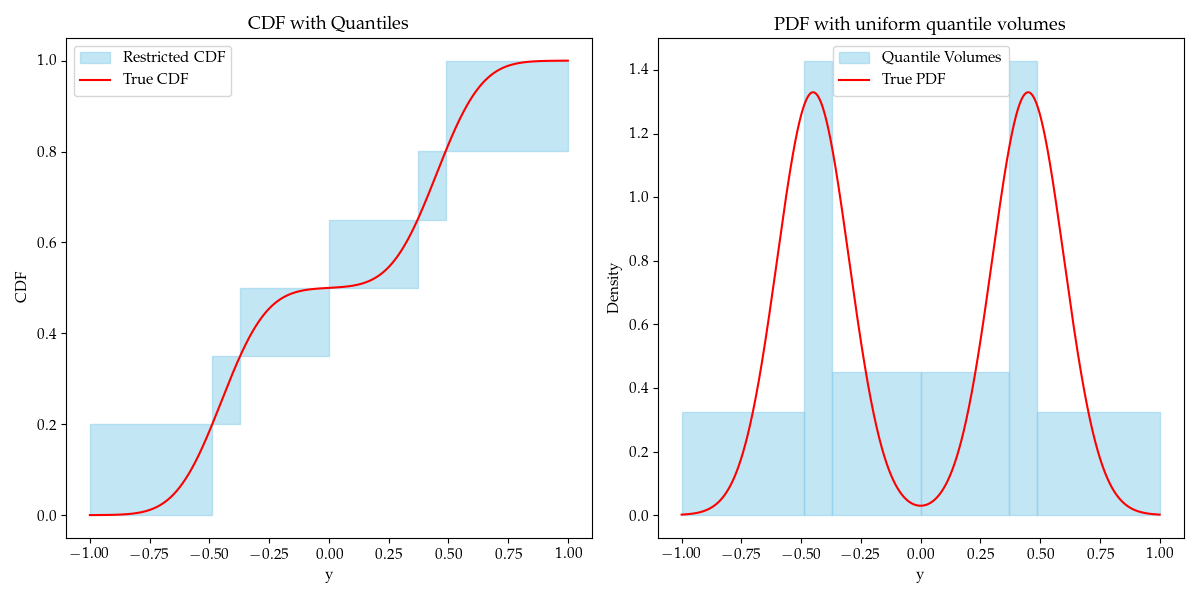
\includegraphics[width=0.8\textwidth]{resources/restricted_pdf_cdf_with_qr5.png}
        \label{fig:restricted_pdf_cdf_with_qr5}
    }\\
    \subfloat[Restricted CDF with 30 quantiles]{
        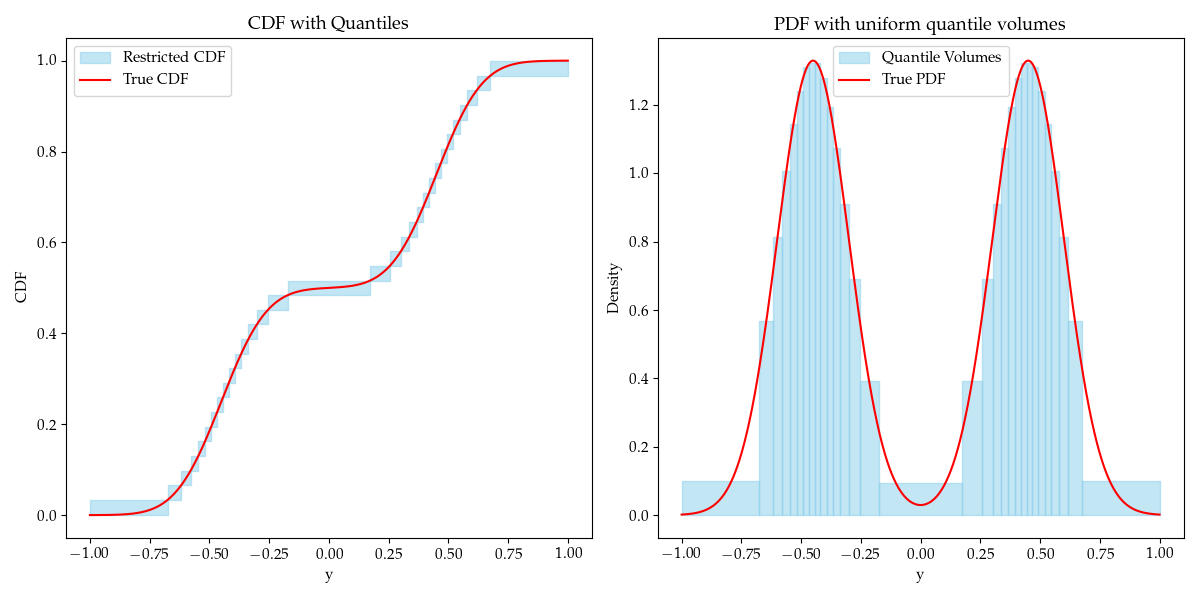
\includegraphics[width=0.8\textwidth]{resources/restricted_pdf_cdf_with_qr30.png}
        \label{fig:restricted_pdf_cdf_with_qr30}
    }

    \caption{We can see that if we increase the number of quantiles that we predict, the restriction on the CDF becomes more and more strict and we approach the true PDF on the right side.}
\end{figure}

We can now infer quite clearly what information is required in a $\mathcal{P}_{\theta}$ in order to do CP, QR or CDE. For QR, we only need to know that $\forall p\in\mathcal{P}_\theta: \int_{-\infty}^{Q(\mathbf{x})} p d\mathbf{y} = q$ for some $q$ which can be also seen in \fef{fig:restricted_pdf_cdf_with_qr5}. Even tho we do not know the full PDF when only looking at the restricted PDF we can still infer certain quantile levels precisely. For CP we need to know that $\forall p\in\mathcal{P}_\theta: \int_{U(\mathbf{x})} p d\mathbf{y} = 1 - \alpha$ for some $\alpha$. In \fef{fig:restricted_pdf_cdf_with_qr5} we can see that this could simply be an interval between two quantile levels that we predict. For CDE we need to know that $\forall p\in\mathcal{P}_\theta: p = p(\mathbf{y} \mid \mathbf{x}; \theta)$. Since for CDE $|\mathcal{P}_\theta| = 1$ it is quite clear that there is no ambiguity in predicting qunatiles or CP regions and we can just choose any quantile or region from the single PDF in $\mathcal{P}_\theta$.

However, in order to be able to obtain $\mathcal{P}_\theta$ such that it is valid for CDE via CP or QR we need to be able to restrict it to be a single element. Therefore, we need to observe that under our standard assumptions %ref
we can just apply multiple QR or CP restrictions to $\mathcal{P}$ by performing multiple CDE-methods that only partially restrict $\mathcal{P}$:

\begin{equation}
    \mathcal{P}_{\theta} = \bigcap_{i=1}^n \mathcal{P}_{\theta_i}
\end{equation}

Where each $\mathcal{P}_{\theta_i}$ is a restriction on $\mathcal{P}$ that is valid for CDE, CP or QR. Thereby one needs to be careful in the definition of each restriction not to have two restrictions that contradict each other and thus produce the empty set, however this is generally approximately possible in practice. What we mean by approximately possible is that we usually can construct a valid PDF from two restrictions that might contradict each other. For example if we do multiple quantile regression and observe quantile inversion, then it is a common practice to simply swap the two quantiles out. In this case in is common practice to just take this then as the final $\mathcal{P}_{\theta}$.\footnote{This common practice, while it results in a valid $\mathcal{P}_{\theta}$ does generally and also in literature lack a theoretical foundation an is more a "trick of the trade". We will not analyze the theoretical validity of doing this.} Moreover, combining restrictions of $\mathcal{P}_\theta$ is already a common method in the literature, e.g. \cite{sesia2021conformal} where multiple quantile regression is used in order to obtain a grid of quantiles that can be used to infer CP regions.

We can arbitrarily restrict $\mathcal{P}_\theta$ if we can make those restrictions arbitrarily tight with a method as we can also see in \fef{fig:restricted_pdf_cdf_with_qr30}. In the case of QR we can simply make an infinitely dense quantile grid which essentially accomplishes that. For CP it is a bit less obvious since we could define CP intervals anywhere and it is unclear how we would make sure that we still restrict everywthing even if we increase/decrease the confidence level. However, all CP methods in the literature (e.g. \cite{sesia2021conformal, chernozhukov2021distributional}) are based on methods that allow for a nested way of increasing/descreasing CP regions which relates to how calibration works in CP as we can see in \pef{sec:calibration}. Nested regions essentially allow that we can make as specific statements about the conditional PDF by interpolating the CP regions.

\subsection{CDE to improve current CP}
In this work we argue, that by first estimating the true conditional density with high precision instead of just restricting it partially we can improve the performance of CP and QR. In particular, by restricting $\mathcal{P}$ more we argue that this provides a regulatory effect where unreasonable partial predictions are purged. This is conceptually similar to the concept of ensembles if we do this by means of multiple quantile regression.

For example, if we were to predict a quantile at a specific position that might not be perfectly accurate, then by having a tight quantile regression grid over the whole space $(0,1)$ we will stabilize this since it is likely in that case that quantile inversion appears and by swapping/sorting the quantiles we can obtain a valid PDF. The same applies to CP.

This implicitly also means that given that the CP/QR method only needs to model a subset of the information of the PDF, it will not worsen the performance if we also try to model other parts of the PDF $\mathcal{P}_{\theta'}$ and use it as regularizer in practice. I.e. if we only want the median then it would not hurt the performance in practice if we also predict the 0.1 and 0.9 quantiles and use them as regularizer.

\subsection{CP methods are practically not distribution free methods}
In the literature it is often argued for the benefit of CP that it is distribution free which means that we do not make any distributional assumptions prior to defining the model. Moreover, if we were to infer CP by means of first estimating a CDE e.g. with a MDN then we on first glance directly make distributional assumptions since a MDN is based on distributional components.

However, even if we introduce distributional assumptions, in fact, it can be shown that when using MDNs for CDE with an infinite number of gaussian components, we can predict any arbitrary PDF and also, in fact, CP methods, when limited to a finite number of model parameters as it is always the case in practice, similarly have distributional assumptions introduced by the modeling limitations of NNs. Those modeling limitations of neural networks are present in the initialization of weights with a certain distribution and the distribution of activations after linearities and activation functions. Each activation function imposes a certain distribution on the model. So both, CP and CDE, are not distribution free methods when limiting the number of model parameters dispite common literature suggesting CP is distribution free. It is generally not true and CP is in the same way distribution in the context of those literature works as CDE is.

\subsection{Limitations of the Bridge between CDE-Methods}

While the statements made about CDE, CP and QR being the same task, they all only directly apply under our standard assumptions. However, even without the standard assumptions, without proof, we reasonably suspect that the same statements basically hold. In those cases it might be that the conditional CDF has discontinuities or flat spots for which of course all three methods will struggle. For example QR might behave strangely since we have a jump in the CDF at this point or on points between the quantile level QR is trying to predict. However, since we can approximate any PDF that does not fullfill our standard assumptions with a PDF that does, we can still argue that the same statements hold approximately and in practice anyways.

Moreover, when combining restrictions on the PDF, current methods, like swapping quantiles with quantiles inversion, to combine them while maintaining a valid PDF are not well studied and also impose assumptions on the PDF which are often quite arbitrary and of practical nature. However, as all CDE-methods are asymptotically consistent, cases where the restrictions contradict are an artifact of limited data and there approximate solutions are used anyways making it not really a limitation. However, it would be good to have a more theoretical foundation for those methods.

\subsection{Conclusion on the Bridge between CDE, CP and QR}

By \pef{sec:bridge_cde_qr} and \pef{sec:bridge_cde_qr} we can see that in the background of each CDE-method the restriction on all PDFs $\mathcal{P}_\theta$ stands. This has two major implications:

Firstly, any technique on a CDE-method also implicitly acts on $\mathcal{P}_\theta$ and thus can be thru $\mathcal{P}_\theta$ translated to any other CDE-method. For example if we were to decide that the std of a CDE model is to be inceased a bit by a particular function, e.g. $f(p) = 2 p $, then this will clearly be reflected in the restricted distribution $\mathcal{P}_\theta$ which means we also could find the generalized form of $f$ which explicitly acts on $\mathcal{P}_\theta$ and thus can be applied to any CDE-method. In this case it would be $f(\mathcal{P}_{\theta}) = \left\{2 p: p \in \mathcal{P} \land \frac{p}{2} \in \mathcal{P}_\theta \right\}$, i.e. we just apply the $f$ to each element in $\mathcal{P}_\theta$. So we see that any technique that acts on a CDE-method can be translated to any other CDE-method.

Secondly, any CDE-method goal can be done with any other CDE-method e.g. we can get a full conditional PDF from a method that does QR or CP.

\section{Optimal Conformal Prediction}\label{sec:optimal_cp}

In this section we first define what we mean by optimal CP and then show how we can infer optimal CP from CDE by using a novel method. We will give a new perspective on the optimization objective of CDE, which often is likelihood, and show how it relates to the definition of optimal conformal prediction that we give here. This relationship is of theoretical interest and also has practical implications as we will show in \pef{sec:calibration}. %make sure thats true

In order to develop our argument we first define what we mean when we say that a CP method is optimal. We orient ourselves on the work of~\cite{sesia2021conformal} where they define the optimal CP method as the one that predicts the shortest intervals for a given miscoverage level $\alpha$. However, instead of only predicing single intervals, we argue that it is simpler and more practical to simply estimate the shortest possible regions of the target space that contain the target variable in expectation with the required confidence level.

Let $\alpha \in (0,1)$ be a significance level. Then the goal of conformal prediction is to find a function $C : \mathbb{R}^n \to \mathcal{B}(\mathbb{R}^m)$ that can predict the subsets with the smallest Lebesgue measure $\lambda$ marginalized over $\Omega$ with significance $\alpha$. That means we want $\mathbb{P}(\mathbf{Y}_I \in C(\mathbf{X}_I)) = 1 - \alpha$ with $\int_{\Omega}\lambda(U(\mathbf{X}_{I(\omega)}(\omega))) d\mathbb{P}(\omega)$ small.

Formulated as a proper constrained optimization problem, we can rewrite the optimization problem as:

\begin{align}
    \min_U \quad      & \int_{\mathbb{R}^{m + n}} p(\mathbf{z})
    \lambda(C(\mathbf{x}))
    d\mathbf{z}
    \\
    \text{s.t.} \quad & \int_{\mathbb{R}^{m + n}} \mathds{1}_{\mathbf{y} \in
    C(\mathbf{x})} d\mathbf{z} = a
\end{align}

\subsection{New perspective on MLL and Optimal CP}\label{sec:optimal_cp_proofs}

The method to infer the intervals that will be used by us is the highest density regions method. Using this method we can, given a PDF, infer the set of intervals with the shortest summed Lebesgue measure. In particular, we are shifting our focus from looking at the shortest regions to looking at the regions that contain the most probability mass, even tho that is very similar and mostly the same with HDR there are some delicate differences. This is partiularly beneficial since regions with high densities should usually not be ignored in practice as they often indecate important events. When only focusing on the shortest possible single interval that contains the desired proportion of probability mass, it might happen that a region with high density is ignored even tho this event might have some core interpretation to domain experts. We argue, that if a single interval is desired it is more beneficial in most domains, to simply take the interval from the small edge of the region of the smallest value to the large edge of the largest value region. This might contain more density than $1 - \alpha$ but we argue that it is in most cases still desirable to design intervals this way. %TODO: need to add some practical proof of that here maybe

If $C$ is being calculated by using first Conditional Density Estimation (CDE) and then using Highest Density Regions (HDRs) as defined by~\cite{hyndman1996computing} to obtain a significance level of $\alpha$, then $C$ is a function of the CDE method and the significance level $\alpha$. HDR is by~\cite{hyndman1996computing} defined as:

\[
    H\left(f_a\right)=\left\{\mathbf{y}: f(\mathbf{y}) \geq f_a\right\}
\]
with
\[
    f_a = \max_{f_a} \left\{f_a \in \mathbb{R^+}: \mathbb{P}\left(\mathbf{y}
    \in
    H(f_a)\right) \geq a \right\}
\]

but it can be written equivalently as below. The below formulation is also the one being used in this work from now on.

\begin{equation}
    H\left(f, a\right):=\left\{\mathbf{y} \in \mathbb{R}^m: f(\mathbf{y}) \geq
    \max_{b} \left\{b \in \mathbb{R^+}: \mathbb{P}\left(\left\{\mathbf{\hat{y}}
    \in
    \mathbb{R}^m: f(\mathbf{\hat{y}}) \geq b\right\}\right) \geq a
    \right\}\right\}
    \label{eq:HDR}
\end{equation}

where $f$ is an arbitrary probability density function (PDF) and $a := 1 - \alpha$ is the confidence level. Note that $\mathbb{P}$ here is different from the one defined in the beginning and only here for defining HDRs. As the CDE method in my case is parametric like mixture density networks it is more reasonable to write $C$ a function of the weights and the significance (and implicitly also the architecture of the CDE of course). So considering that, the initial goal of conformal prediction can be rewritten as:

\begin{align}
    \min_{\theta \in \Theta} \quad & \int_{\mathbb{R}^{m + n}} p(\mathbf{z})
    \lambda(H(p(\mathbf{\hat{y}} \mid \mathbf{x}; \theta), a))
    d\mathbf{z}
    \\
    \text{s.t.} \quad              & \int_{\mathbb{R}^{m + n}}
    \mathds{1}_{\mathbf{y} \in
    H(p(\mathbf{\hat{y}} \mid \mathbf{x}; \theta), a)} d\mathbf{z} = a
\end{align}

where it is important that the $\mathbf{\hat{y}}$ is not the one we integrate over but more a demonstrative artefact we write to denote that $p(\mathbf{\hat{y}} \mid \mathbf{x}; \theta)$ is a conditional density. Moreover $\Theta$ is the space of all parameters of the CDE method.

In the following if we write $p(\mathbf{\hat{y}} \mid \mathbf{x}; \theta)$ we mean a conditional density estimator parameterized with $\theta$ which implicitly contains the architecture and the weights of the method and if we write $p(\mathbf{\hat{y}} \mid \mathbf{x})$, the true conditional density is meant. Notice, that the goal of this optimization problem is to optimize w.r.t. $\theta$ as it is basically the component that completely defines $p(\mathbf{\hat{y}} \mid \mathbf{x}; \theta)$. This in turn means we need to find the argmin of the
optimization above.

Let $\theta^*$ be the argmin of the equation above, we would like to show that

\begin{equation}
    \theta^* = \argmax_{\theta \in \Theta}  \int_{\mathbb{R}^{m + n}}
    p(\mathbf{z}) \log p(\mathbf{y} \mid \mathbf{x}; \theta) d
    \mathbf{z}
\end{equation}

which is the maximum likelihood estimator (MLE). This is of great importance if we wish to optimize a CDE method w.r.t. the maximum likelihood objective function in order to implicitly optimize for the conformal prediction objective function when using HDRs. In order to show this powerful statement we first need to develop some insight into the workings of the components in conformal prediction.

First, we require to show that $\lambda(H(p, a))$ is continously differentiable a.e. in order to make sensible statements. Its not that the intuition does not hold if its not continous, however, it complicates things and makes the statemtent more difficult. First in \sref[Lemma]{lem:continuity} below we show that this is fullfilled if the PDF fullfills our standard assumptions in \sref[Assumptions]{def:assumptions}.

Note that the second assumption is fullfilled if it holds that $p$ is changing a.e. or the area with derivative $0$ is of measure $0$ which is left without proof. %TODO: maybe reference to some measure theory book

\begin{lemma}\label{lem:continuity}
    Let \(p: \mathbb{R}^m \to \mathbb{R}\) be a probability density function for which \sref[Assumptions]{def:assumptions} hold where we neglect the $\mathbf{x}$ for breefity.

    Furthermore let $p$ be for the random variable $\mathbf{Y}$ (for breefity we neglect the index) and let $g(b) := \mathbb{P}(p(\mathbf{Y}) \geq b)$. Moreover, $\lambda_p:[0, 1] \to \mathbb{R}$ with $\lambda_p(a) = \lambda(H(p, a))$. Then the following statements hold for $a \in (0,1)$:

    \begin{enumerate}
        \item $g(b)$ is strictly monotonic on the set $g^{-1}((0,1))$.
        \item $g(b)$ is continous.
        \item $g(b)$ is bijective on the set $g^{-1}((0,1))$.
        \item $g(b)$ is continously differentiable a.e. %-> todo
        \item $B(p, a)$ is strictly monotonous on the set $B^{-1}((0,1))$.
        \item $B(p, a)$ is continous.
        \item $B(p, a)$ is bijecitve on the set $B^{-1}((0,1))$.
        \item $B(p, a)$ is continously differentiable a.e. % todo
        \item $\lambda_p(a)$ is strictly monotonous.
        \item $\lambda_p(a)$ is continous.
        \item $\lambda_p(a)$ is bijective on the set $\lambda_p^{-1}((0,\infty))$.
        \item $\lambda_p(a)$ is continously differentiable a.e. %todo
    \end{enumerate}
\end{lemma}

It is in particular required to not have any flat-splots in the PDF because otherwise per definition of HDR we can sometimes not obtain the shortest possible intervals for a confidence level $a$ since we would not know which part of the flat-spot to include in the interval and which to leave out. In practice this would hardly be a problem.

\begin{proof}
    1. Monotonicity itself is obvious since we can not make the set $\mathbf{Y} \geq b$ larger when increasing $b$. For strict monotonicity on $g^{-1}((0,1))$ we require that $\forall b \in g^{-1}((0,1)): \frac{\partial \mathbb{P}(p(\mathbf{Y}) \geq b)}{\partial b} > 0$.

    Let $b$ be in $g^{-1}((0,1))$. We essentially need to show that for any $b' > b$ there exists a $\epsilon > 0$ such that $\mathbb{P}(p(\mathbf{Y}) \geq b + \epsilon) = \epsilon + \mathbb{P}(p(\mathbf{Y}) \geq b')$ which essentially means that there is change in $g$ no matter how tight we choose the interval which comes directly from the definition of the derivative. So let $b'$ be like so, and choose any $b'' \in (b, b')$, then continuity of $p$ implies there exists a dense neighborhood around $b''$ which lies in $p(\mathbf{Y}) \in (b, b')$. In particular the fact that this neighborhood is dense also implies via the Lebesgue Density Theroem that this neighborhood has a positive Lebesuge measure and the assumption that $p > 0$ implies that it does also have positive probability measure. This implies the result of strict monotonicity.

    2. To show continuity of $g$ we use that it is because of monotonicity and boundedness of the $\mathbb{P}$ measure, that for any $\tilde{b}\in\mathbb{R}^+$

    \begin{equation}
        \lim_{b \downarrow \tilde{b}} g(b) = \mathbf{P}(\mathbf{Y} > \tilde{b})
    \end{equation}

    and also

    \begin{equation}
        \lim_{b \uparrow \tilde{b}} g(b) = \mathbf{P}(\mathbf{Y} \geq \tilde{b})
    \end{equation}

    where implicitly the continuity of $p$ from above and below are used. This means the two limits are always the same if $\mathbb{P}{\mathbf{Y} = \tilde{b}} = 0$ which is an assumption and thus continuity of $g$ is shown.

    3. Bijectivity follows from strict monotonicity directly. To be exact why actually $g^{-1}((0,1))$ exists for every $a \in (0,1)$ we can use the monotonicty of $g$ and the intermediate value therem since we can clearly find a $b$ such that $g(b)$ is arbitrarily close to $0$ and to $1$ because of the PDF property of $p$ and the fact that continuity of $p$ implies boundedness of $p$.

    4. Differntiability a.e. follows from the Lebesgue's Theorem for Monotonic Function as $g$ is monotonic. Continous differentiability a.e. follows from the fact that $g$ is uniformly continous due to the Heine-Cantor Theorem and this implies that the derivative is continous a.e. as well. %might want to go more into detail here but maybe its not necessary

    5. This follows by observing that $g$ is bijective on $g^{-1}((0,1))$ which implies that the maximum of $b$ where $g$ is still greater-equal $a$ will always exactly reach $a$. Then since $g$ is $g^{-1}((0,1))$ is well defined and $g$ is strictly monotonic we see that increasing $a$ will always increase the possible $b$.

    6. Continuity follows from the fact that $g$ is also continous and bijective.

    7. Bijectivity follows directly from 5. and 6. similar to 3.

    8. Follows with the same logic as 4.

    9. Strict monotonicity of $B$ and the same argument as in 1. (Lebesgue density theorem) imply this.

    10. This can also be shown by the same argument as 2. and continuity of $B$ in 6.

    11. Bijectivity follows from 9. The fact that the image is $(0,\infty)$ follows from the fact that $p>0$ and thus in order to go with $a \to 1$ we will require infinite area in the Lebesgue sense. That we also approach $0$ in the image follows easily from bijectivity of $B$ on $(0,1)$.

    12. Follows with the same logic as 4.
\end{proof}

From this lemma we can see that iff the PDF is continously diffentiable a.e., also the length of the HDR w.r.t. $a$ will be continously differentiable a.e.. This is required because otherwise we can not show the following lemma about convexity of the HDR length w.r.t. $a$:

\begin{lemma}
    Let \(p: \mathbb{R}^m \to \mathbb{R}\) fullfill the Assumptions~\ref{def:assumptions}. Then, the function \(\lambda_{H_p}(a) := \lambda(H(p, a))\), representing the size of the highest density region (HDR) for PDF \(p\) with coverage \(a\), is strictly convex, i.e.,

    \begin{equation}
        \frac{\partial^2 \lambda_{H_p}(a)}{\partial a^2} > 0.
    \end{equation}

\end{lemma}
\begin{proof}
    Without loss of generality, assume \(a_1 < a_2\) with both \(a_1, a_2 \in (0,1)\). For any \(\alpha \in (0, 1)\), let \(a := \alpha a_1 + (1-\alpha) a_2\). By the definition of \(H_p\) in \eef{eq:HDR}, the set \(H(p, a)\) encompasses points up to the highest densities corresponding to coverage \(a\). Taken from the definition in \eef{eq:HDR} we define this highest density as

    \begin{equation}
        B(p, a):=\max \left\{b \in \mathbb{R^+}: \mathbb{P}\left(\left\{\mathbf{\hat{y}}
        \in
        \mathbb{R}^m: p(\mathbf{\hat{y}}) \geq b\right\}\right) \geq a
        \right\}
    \end{equation}

    This implies that \(\lambda_{H_p}(a_1) \leq \lambda_{H_p}(a) \leq \lambda_{H_p}(a_2)\). Define $k_1 = a-a_1$, $k_2 = a_2 - a$. Consequently, \(H(p, a_1) \subset H(p, a)\), indicating that to transition from \(H(p, a_1)\) to \(H(p, a)\), only points with density less than $B(p, a_1)$ can be utilized. In contrast, if we go from $a$ to $a_2$ only points with a density less than $B(p, a)$ can be utilized.

    As we know that
    \begin{equation}
        \lambda_p(a) = \lambda(H(p, a)) = \lambda(H(p, a_1) \cup (H(p,a)\setminus H(p,a_1))) = \lambda(H(p, a_1)) + \lambda(H(p,a)\setminus H(p, a_1))
    \end{equation}
    and we know that $\lambda(H(p,a)\setminus H(p, a_1)) \leq k_1 \cdot B(p, a)$ and $\lambda(H(p,a_2)\setminus H(p, a)) \geq k_2 \cdot B(p, a)$ we can finally see that we can approximate the gradient by dividing the change of $\lambda_p$ by the change of $a$, which is in $k_1$ and $k_2$ we see that the gradients are bounded from above and below respectively for the invervals $(a_1, a)$ and $(a, a_2)$. Moreover strict monotonicity of $B$ as shown in Lemma~\ref{lem:continuity} implies that the gradient is strictly increasing for $\lambda_p$ which implies a postive second derivative and thus convexity.

    In particular, the second derivative exists by the use of the Lebesgue's Theorem for Monotonic Function a.e. since the first derivative exists continuously a.e. and is strictly monotonic as we know from \sref[Lemma]{lem:continuity} which implies absolute continous derivative a.e. and thus twice differentiability a.e..
\end{proof}

\begin{lemma}\label{lem:hdr_optimality_mll}
    For any PDFs $f: \mathbb{R}^m \to \mathbb{R}$ and $p: \mathbb{R}^m \to \mathbb{R}$, where $p$ must fullfill \sref[Assumptions]{def:assumptions}, with the same coverage size under confidence levels $a_p$ and $a_f$, that is,

    \[\lambda(H(f, a_f)) = \lambda(H(p,a_p))\]

    it holds that if we measure the coverage of those HDRs with points distributed w.r.t. $p$, that the coverage measured with $H(p,a)$ will be greater-equal. Moreover, the coverage level of $H(p,a)$ will be exactly $a_p$. Formally:

    \[
        \int_{\mathbb{R}^{m}} p(\mathbf{y}) \mathds1_{\mathbf{y} \in H(f, a_f)} d
        \mathbf{y} \leq \int_{\mathbb{R}^{m}} p(\mathbf{y})
        \mathds1_{\mathbf{y} \in
            H(p, a_p)} d \mathbf{y} = a_p
    \]
\end{lemma}
Note that it is absolutely possible that $a_p = a_f$.
\begin{proof}
    We split $H(p,a_p)$ and $H(f, a_f)$ into subsets: $H(f, a_f) = A \cup B$ and $H(p, a_p) = A \cup C$ with $H(f, a_f) \cap H(p,a_p) = A$, $H(f, a_f)\setminus A = B$ and $H(p, a_p)\setminus A = C$.

    \begin{equation}
        \int_{\mathbb{R}^{m}} p(\mathbf{y}) \mathds1_{\mathbf{y} \in H(f, a_f)} d
        \mathbf{y} = \int_{H(f, a_f)} p(\mathbf{y}) d \mathbf{y} = \int_{A}
        p(\mathbf{y})
        d \mathbf{y} + \int_{B} p(\mathbf{y}) d \mathbf{y}
    \end{equation}

    \begin{equation}
        \int_{\mathbb{R}^{m}} p(\mathbf{y}) \mathds1_{\mathbf{y} \in H(p, a_p)} d
        \mathbf{y} = \int_{H(p, a_p)} p(\mathbf{y}) d \mathbf{y} = \int_{A}
        p(\mathbf{y})
        d \mathbf{y} + \int_{C} p(\mathbf{y}) d \mathbf{y}
    \end{equation}

    since the $A$ part of the integrals is equal we can ignore it for comparing $H(f, a_f)$ and $H(p, a_p)$ coverage. So, we need to show:

    \begin{equation}
        \int_{B} p(\mathbf{y}) d \mathbf{y} \leq \int_{C} p(\mathbf{y}) d
        \mathbf{y}
    \end{equation}

    This can be shown by proofing $\forall \mathbf{y}_B\in B \forall \mathbf{y}_C \in C: p(\mathbf{y}_B) \leq p(\mathbf{y}_C)$ because $\lambda(B) =  \lambda(C)$.
    So, let $\mathbf{y}_B$ and $\mathbf{y}_C$ be arbitrary from the corresponding sets. Then we know that $\mathbf{y}_B \in H(p,a_p)$, which means that $p(\mathbf{y}_C) \geq B(p, a_p)$ where $B(p, a_p)$ is the maximum density bound such that the coverage level of $a_p$ is still given w.r.t. $p$. However, since $\mathbf{y}_C \notin H(p,a_p)$ this means that $p(\mathbf{y}_C) < B(p, a_p)$, which shows the first part of the proof.

    The second part of the proof is to show that
    \begin{equation}
        \int_{\mathbb{R}^{m}} p(\mathbf{y}) \mathds1_{\mathbf{y} \in H(p, a_p)} d
        \mathbf{y} = a_p
    \end{equation}

    which follows from the fact that with our Assumption~\ref{def:assumptions} $B(p, a_p)$ is bijective and thus $\mathbb{P}(\mathbf{Y} \geq B(p, a_p)) = a_p$. In particular, $H(p, a_p)$ is per construction a set where this is fullfilled.
\end{proof}

In order to finally be able to use this lemma efficiently we need to define something like an inverse of the HDR w.r.t. the significance, which based on the input $\mathbf{x}$ and the length $\lambda(H(p(\mathbf{y} \mid \mathbf{y}), a))$ gives us the significance level that we would need to insert in $H$ together with the true distribution at $x$ to obtain the same size of the distribution but with the above lemma always has a larger or equal coverage.

\begin{definition}[HDR Transform]\label{def:hdr_transform}
    Let $f,p : \mathbb{R}^m \to \mathbb{R}$ be two probability density functions and let $a \in (0,1)$ be some coverage level. Then we define the HDR Transform as:

    \[
        H_p(f, a) = \argmax_{b \in (0,1)} \lambda(H(p, b)) \leq \lambda(H(f, a))
    \]

\end{definition}
In words, the HDR Transform gives us the maximal significance level that we can insert under the distribution $p$ while maintaining a coverage size lower-equal than what we obtain by inserting the significance level $a$ under the distribution $f$.

In particular, if we evaluate the actual coverage of $H(f, a)$ with samples drawn from $p$, then the coverage will be always lower-equal $a$ which follows from Lemma~\ref{lem:hdr_optimality_mll}. The HDR transform then gives us basically the confidence level that we need to insert into the HDR with the true distribution to obtain the same coverage size but are guranteed to have higher-equal coverage.

Using this definition together with Lemma~\ref{lem:hdr_optimality_mll} establishes a very powerful tool to make proofs related to HDR.

\begin{lemma}\label{lem:hdr_optimality}
    With $f,p$ as in Definition~\ref{def:hdr_transform} and Assumptions~\ref{def:assumptions} on $p$, it always holds that:

    \begin{equation}
        H_p(f, a) = \argmax_{b \in (0,1)} \lambda(H(p, b)) \leq \lambda(H(f, a)) = \argmax_{b \in (0,1)} \lambda(H(p, b)) = \lambda(H(f, a))
    \end{equation}
\end{lemma}
\begin{proof}
    Bijectivity of $\lambda_p(a)$, under the assumptions, with Lemma~\ref{lem:continuity} implies that exactly one $b$ exists such that $\lambda(H(p, b)) = \lambda(H(f, a))$ which finishes the proof.
\end{proof}

Now we have all tools in order to proof the important statement. From now on, if the expectation $\mathbb{E}$ is used, it is always w.r.t. the whole space $\mathbb{R}^{m+n}$ and with the random variables $\mathbf{Y}$ and $\mathbf{X}$ which have PDF $p(\mathbf{y}, \mathbf{x})$. Moverover, if $\mathbf{\hat{y}}$ is written, it is not an input to the function but a demonstrative artefact to show that the function maps to a conditional density on the same space as $\mathbf{Y}$ is defined.

\begin{theorem}[MLL is equivalent with Optimal Conformal Prediction]\label{thm:optimal_cp}
    We want to show that if we have definitions as in \pef{sec:cp}, the space of all parameters $\Theta$ and $\forall \mathbf{x}\in\mathbb{R}^n: p(\mathbf{y}\mid \mathbf{x})$ fullfills Assumptions~\ref{def:assumptions} and that $\forall \mathbf{x}\in \mathbb{R}^n: \max_{\theta} p(\mathbf{y} \mid \mathbf{x}; \theta) = p(\mathbf{y} \mid \mathbf{x})$, then it holds that:

    \begin{equation}
        \argmax_{\theta \in \Theta}  \mathbb{E} \left[ \log
            p(\mathbf{Y} \mid \mathbf{X}; \theta) \right]
    \end{equation}

    equals

    \begin{align}
         & \argmin_{\theta \in \Theta} \mathbb{E} \left[
            \lambda(H(p(\mathbf{\hat{y}} \mid \mathbf{X}; \theta), a))
        \right]                                          \\
         & \text{s.t.} \quad \mathbb{E} \left[
        \mathds{1}_{\mathbf{Y} \in
        H(p(\mathbf{\hat{y}} \mid \mathbf{X}; \theta), a)} \right]
        = a
    \end{align}

\end{theorem}

\begin{proof}
    For brevity, let $H_{\theta} := H(p(\mathbf{\hat{y}}\mid \mathbf{X}; \theta), a)$ and $H_{\mathbf{\Theta^*}} := H(p(\mathbf{\hat{y}}\mid \mathbf{X}; \theta^*), a)$.

    In this case let's assume that now we have some $\theta \neq \theta^*$. We can show that if for this $\theta$ it holds that if

    \begin{equation}
        \mathbb{E} \left[ \lambda(H_{\theta})\right]
        <
        \left[\lambda(H_{\mathbf{\Theta^*}}) \right]
    \end{equation}
    it implies
    \begin{equation}
        \mathbb{E} \left[ \mathds{1}_{\mathbf{Y} \in
        H_{\theta}} \right] < a
    \end{equation}

    which would finish the proof, since it'd show that for any parameter set $\theta$, that produces a smaller average HDR than the the MLE, the constraint would be violated and it is clear that if using the MLE, which is the same as the true PDF, we would fulfill the constraint because of Lemma~\ref{lem:hdr_optimality_mll}.

    First, we can upper bound the coverage with the IH:

    \begin{equation}
        \mathbb{E} \left[ \mathds{1}_{\mathbf{Y} \in
        H_{\theta}} \right]
        \leq
        \mathbb{E} \left[ \mathds{1}_{\mathbf{Y} \in
        H(p(\mathbf{\hat{y}} \mid \mathbf{X}), IH(p(\mathbf{\hat{y}}\mid
        \mathbf{X};
        \theta), a))} \right]
        \label{eq:upper_bound}
    \end{equation}

    \begin{equation}
        = \mathbb{E}\left[IH(p(\mathbf{\hat{y}}\mid \mathbf{X}; \theta),
            a)
            \right]
        \label{eq:upper_bound_2}
    \end{equation}

    The upper bound follows directly from Lemma~\ref{lem:hdr_optimality_mll} and the monotonicity property of integrals. The equality in \eef{eq:upper_bound_2} follows from the fact that if we evaluate the coverage w.r.t. underlying distribution $p$ we will always get the same coverage level as the one we inserted in the HDR if we fullfill Assumptions~\ref{def:assumptions}.

    We know that:
    \begin{equation}
        \mathbb{E}\left[\lambda(H_{\mathbf{\Theta^*}})\right] > \mathbb{E}\left[ \lambda(H_{\theta}) \right]
        \label{eq:inequality_0}
    \end{equation}
    and
    \begin{equation}
        \mathbb{E}\left[ \lambda(H_{\theta}) \right]
        =\mathbb{E}\left[ \lambda(H(p(\mathbf{\hat{y}}\mid\mathbf{X}),
            IH(p(\mathbf{\hat{y}}\mid \mathbf{X}; \theta), a)))
            \right]
        \label{eq:inequality_1}
    \end{equation}

    where the second equality follows from Lemma~\ref{lem:hdr_optimality}. This upper bound gives via Lemma~\ref{lem:hdr_optimality} the highest coverage level for the same coverage size that is possible. If we can show the desired result for this upper bound, then we have shown the desired result.

    Due to convexity and with the Jensen inequality we can now show that then we have appended to the equation in \eef{eq:inequality_1} the following inequality:
    \begin{equation}
        \geq \mathbb{E}\left[ \lambda(H(p(\mathbf{\hat{y}}\mid\mathbf{X}),
            \mathbb{E}\left[IH(p(\mathbf{\hat{y}}\mid \mathbf{X};
                \theta), a)
                \right] ))\right]
    \end{equation}

    and thus:

    \begin{equation}
        \mathbb{E}\left[\lambda(H(p(\mathbf{\hat{y}}\mid
            \mathbf{X}),a)))\right]
        > \mathbb{E}\left[ \lambda(H(p(\mathbf{\hat{y}}\mid\mathbf{X}),
            \mathbb{E}\left[IH(p(\mathbf{\hat{y}}\mid \mathbf{X};
                \theta), a)
                \right] ))\right]
    \end{equation}

    In words, what this means is that given the same distribution $p(\mathbf{\hat{y}}\mid\mathbf{x})$, we obtain a strictly larger average coverage size when using coverage $a$, then when we use coverage $\mathbb{E}\left[IH(p(\mathbf{\hat{y}}\mid \mathbf{x};\theta), a)\right]$. By monotonicity of the coverage size function, this means a.e. that

    \begin{equation}
        \lambda(H(p(\mathbf{\hat{y}}\mid\mathbf{X}),a))) > \lambda(H(p(\mathbf{\hat{y}}\mid\mathbf{X}),
        \mathbb{E}\left[IH(p(\mathbf{\hat{y}}\mid \mathbf{X};
            \theta), a)
            \right] ))
    \end{equation}

    since it can a.e. not be that the inequality is reversed, and thus:

    \begin{equation}
        a > \mathbb{E}\left[IH(p(\mathbf{\hat{y}}\mid \mathbf{X};\theta), a)\right]
    \end{equation}

    which, as we can see in \eef{eq:upper_bound}, upper bounds the coverage of the actual $p(\mathbf{\hat{y}}\mid \mathbf{X};\theta)$. This completes the proof.

\end{proof}
This now shows our desired result, that in fact, by maximizing the likelihood of a CDE model to afterwards apply HDR to obtain small but calibrated regions is equivalent to directly trying to minimize the size of the HDR while maintaining calibration. When assuming that our CDE models can reasonably well approximate the true underlying distribution this is a powerful result that allows us to focus fully on optimizing the likelihood for CDE and we get optimal conformal prediction with HDR for free.

Moreover, we can see that this means the MLE can be decomposed into a constrained optimization problem. In particular this is true because not only the MLE is the ideal model for optimal CP, but also the inverse is true, the optimal CP model is also the optimal MLE model which follows directly from the equality that was just shown in \sref[Theorem]{thm:optimal_cp}. While in the context of this work we leave it as a theoretical insight, it is possible that this can be used in future work for new relevant findings. Arguably this fact has some mathematical beauty to it, as we realize the MLE inherently is looking for the tightest possible peaks while maintaining calibration. %maybe leave this subjective part out even though it is true

\subsection{Focusing on Density instead of the Coverage Level}\label{sec:density_focus}

AS hinted in \pef{sec:motivation} in this work we argue that it is practically more reasonable to move the focus to the probability mass/density instead of only the length of the inverval while maintaining calibration. The difference is subtle, but via \fef{fig:hdr_vs_shortest_intervals} we hope to give some intuitive understanding of the difference with two different arguments.

Firstly, we are when doing CP only focusing on the length of the single inverval being as short as possible in the prediction while maintaining calibration entriely argnostic to the actual shape of the distribution. In particular, if it were possible to obtain significantly more mass with just a very slight increase the interval size it would be ignored. In the figure this can be observed when comparing the connected HDR with the shortest interval CP. We can see that when we first use HDR but then simply connect it, with the argumentation of \cite{sesia2021conformal} (multiple intervals can be confusing in practice), we will capture the second peak of the distribution while we do not capture low density parts of the first bigger peak. This is a clear example of where focusing on the length of the interval can be misleading.

Secondly, another intutive reason, even tho we lack empirical evidence of this, why a second predicted peak should be included in the CP prediction is that it appears reasonable to us that if the model learned a second spiky modality at a specific point than there must be a good reason therefore whilst a heavy tail might simply be an artifact of the modeling method. We are looking for further research to confirm this hypothesis.

Primarely for the first but also for the second reason, we believe that when using our approach (first HDR then connect regions) that it is of advantage in practical scenarios like healthcare and fincance.

\begin{figure}
    \centering
    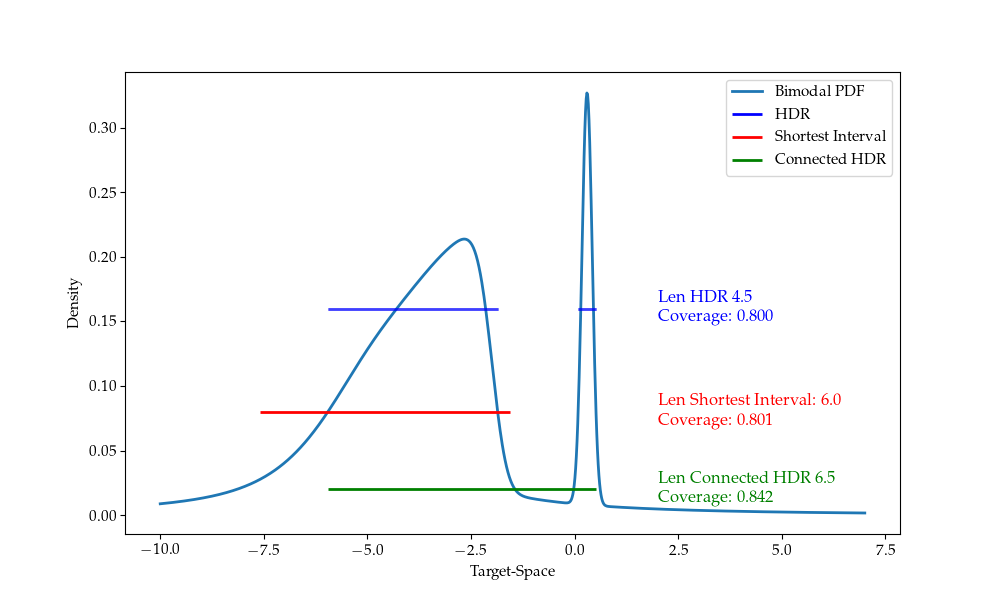
\includegraphics[width=0.8\textwidth]{resources/bimodal_distribution_hdr_vs_shortest_interval.png}
    \caption[Comparison of HDR, connected HDR and Shortest Interval CP]{Comparison of HDR, connected HDR and Shortest Interval CP for a bimodal distribution. We can see that although the connected HDR slightly overcoveres, we obtain significantly more coverage with only a slightly larger interval and also intutively this interval is more meaningful.}
    \label{fig:hdr_vs_shortest_intervals}
\end{figure}

%\section{Time series forecasting Theory}\label{sec:forecasting}

\section{Calibration and Recalibration}\label{sec:calibration}

CDE-methods, while calibrated when optimal, in practice are often not calibrated due to model misspecification, overfitting or underfitting. Calibration if the model is optimal directly follows from the fact that under our assumption the optimal model is the true PDF and the true PDF is calibrated of course. For this section of our work we assume a limited training set $\mathcal{Z} = (\mathcal{X}, \mathcal{Y})$ that is used to train the CDE-method model. The probably most important realization on this is, that even tho the objective functions CDE-methods use in practice are optimal in theory, in practice we mostly need to resort to gradient based optimization methods, which require a step wise optimization and will only find local optima. Especially this insight is important because that means, even tho globally optimal models w.r.t. objective functions of CDE-methods will be calibrated, those objective functions do not gurantee calibration at all times during optimization. The reason is that the constraint of those optimization problems is an implicit one in practice and we will violate it usually with CP.% Moreover, another important insight is that due to the limited amount of data we have, we also usually have to make heavy smoothness assumptions as described in \pef{sec:smoothness}.

This is the reason why in practice recalibration methods exist and are at this time mostly applied to CP methods. From \pef{sec:cp_sub_cde} it follows that we can apply the same methods to all CDE-methods that are used currently only for CP. However, since recalibration methods are mostly explored in CP methods, we will first introduce them in the context of CP in \pef{sec:calibration_cp} and step-wise extend the methods till we reach full generalization of recalibration in all CDE-methods in \pef{sec:calibration_cde_general}.

\subsection{Calibration in CP}\label{sec:calibration_cp}
Generally, calibration of CP refers to the requirement of the defining property of CP to be fullfilled as described in \pef{sec:cp}. In particular, since today most CP methods don't aim to estimate any CP intervals but specific ones, during optimization the calibration requirement is often overshadowed. However, calibration in the context of CP is basically the whole point of CP to begin with and because it is in practice often not fullfilled, recalibration methods are employed.

In any case, if doing recalibration we have that the estimated conformal intervals do in expectation not capture the desired $1 - \alpha$ proportion of the target in the calibration set. However, this can be tackled by recalibration for which a large possible number of methods exist, each depending on the method used to estimate the CP intervals.

One can view the marginal calibration itself as a optimization problem where the objective function is defined as:
\begin{equation}
    \min |(1 - \alpha) - \mathbb{P}(\mathbf{Y} \in C(\mathbf{X}, \psi))|
    \label{eq:calibration_objective}
\end{equation}
, where $C$ is a map to the CP regions. $\psi\in\Psi$ is a configuration of the method used that can be optimized w.r.t. objective function and can be quite arbitrary. In particular, $\psi$ is not generally the same the parameters of the CDE-method model that has been estimated but rather it is something that we apply after the CDE-method model has been estimated. We usually assume that we already have learned a CDE-method model estimated with parameters $\theta$ but that it is possibly not calibrated. One can better understand this by realizing that \pef{sec:cp_sub_cde} implies that any CDE-method can be used to estimate CP intervals and every CDE-method implicitly can fully model the true PDF in the sense that we can restrict $\mathcal{P}_{\theta}$ arbitrarily close to the true PDF. In particular, we can with that see that we need to reformulate \eef{eq:calibration_objective} to:

\begin{equation}
    \min |(1 - \alpha) - \mathbb{P}(\mathbf{Y} \in C(\mathcal{P}_{\theta}, \psi))|
    \label{eq:calibration_objective_formal}
\end{equation}

if we want to be perfectly rigorous since all CP methods necissarly act on a restricted subset of all possible PDFs as discussed in \pef{sec:cp_sub_cde}. Now we also observe that $C$ can be very arbitrary, very much dependent on the exact form of $\mathcal{P}_{\theta}$. For example if from $\mathcal{P}_{\theta}$ we only know a single quantile in terms of restriction, then we can only define a CP interval between $- \infty$ and this quantile and $\Psi$ is essentially the empty set, i.e. $C$ is not parametric in this case. We can see, that without of further assumptions we will not come very far. In particlar, we have no way of minimizing \eef{eq:calibration_objective_formal} without further assumptions since the only thing we know about $\mathcal{P}_\theta$ is a single quantile and this if we are not calibrated this quantile appears to be wrong. Further, without more assumptions we can not simply change $\mathcal{P}_\theta$ as this is the all we know about the true conditional PDF. Moreover, even if the CDE-method used is very restrictive in terms of $\mathcal{P}_{\theta}$, for example $|\mathcal{P}_{\theta}|=1$, then we still can not simply change $\mathcal{P}_{\theta}$ if we are not calibrated since the fact that we are not calibrated indicates that the learned $\mathcal{P}_{\theta}$ is invalid. The question arises what gives us the right to simply manipulate $\mathcal{P}_{\theta}$, which we are already doing in practice as an abundance of current literature shows \cite{}.

What appears to be a reasonable assumption is that while $\mathcal{P}_{\theta}$ might be a restriction that is not correct, we might want to assume that it is close to what is correct; Possibly that the KL-divergence is low between each element of $\mathcal{P}_{\theta}$ and the true conditional PDF, that is lower than for a randomly choosen PDF. The reason why this closeness is reasonably to assume is that all CDE-methods implicitly gurantee asymptotic optimality in the very definitions of their objective functions.

n any case, current literature provides methods that, based on the estimated $\mathcal{P}_{\theta}$, lets us estimate calibrated CP intervals which are close in some sense to the uncalibrated intervals, i.e. the calibrated $\mathcal{P}_{\theta}$ is close to the uncalibrated. Before we go into the details in \pef{sec:implicit_assumptions_cp} and later sections what it means for a calibrated $\mathcal{P}_{\theta}$ to be close or how this can be interpreted in the whole scale of the restricted set of all conditional PDFs $\mathcal{P}_{\theta}$, we will first introduce the methods that are used in practice to recalibrate CP intervals.
%TODO: need to be very careful with assns
%we can basically choose between many different variations of $\psi$ which means that in this case we can optimize this objective very well.

In the following we will describe a variation of $C$ and $\theta$ where we simplify the optimization problem in \eef{eq:calibration_objective_formal} to one that we can practically easily optimize. The method we focus on here is heavily inspired by~\cite{sesia2021conformal} and can be used if $C$ and $\theta$ fullfill certain properties.

\begin{enumerate}\label{list:recalibration_requirements}
    \item $U(,\psi)$ must be such that $\left(U\left(\cdot, \psi_r\right)\right)_{r \in \mathbf{R} \subsetneq \mathbb{R}}$ where $\mathbf{R}$ is bounded and $(U(\cdot,\psi_r))$ are strictly nested sets on the target space where the smallest set $(U(,\psi_0)) = \emptyset$ is the empty set and the largest one contains the full target space. I.e. we have $\forall r_1, r_2 \in \mathbf{R}: r_1 < r_2 \implies U(\cdot,\psi_{r_1}) \subset U(\cdot, \psi_{r_2})$.
    \item We require that the sequence is continous in a way if we want to be able to gurantee that we can come arbitrarily close the the desired calibration in expectation. I.e. $\forall a\in(0,1) \exists \psi\in\Psi : a = \mathbb{P}(\mathbf{Y} \in C(\mathcal{P}_{\theta}, \psi))$
\end{enumerate}

If condition 2 in~\ref{list:recalibration_requirements} is not fullfilled we can only gurantee that the calibration in expectation will be larger-equal the desired proportion. When condition one is not fullfilled, we can not gurantee anything about the calibration in expectation, not even that it will be larger-equal the desired proportion. This is because there might be sets that are never part of the sequence but contain probability mass and thus we can never gurantee that we come even close to the desired calibration in expectation there.

If we optimize \eef{eq:calibration_objective_formal} on the calibration set we can gurantee that the model is calibrated in expectation on the calibration set when assuming exchangability. Moreover, if we do not have set-continous nested sets, we can still gurantee in expectation that the CP interval has a larger-equal converage than the desired confidence level by simply taking $r$ such that $(1 - \alpha) - \mathbb{P}(\mathbf{Y} \in U(\cdot, \psi))$ is still negative and minimal in absolute value.

%TODO: add proof that this is the case

The method used by \cite{sesia2021conformal, chernozhukov2021distributional} is to basically sort the $r$ that are required for each of the calibration samples to be included in the CP interval. Then we take the upper $(1- \alpha)$ quantile of this sorted list as the $r$ that we use for the CP interval. We refer to \cite{sesia2021conformal} for a more detailed explanation of the method and of it's validity, but it gurantees in expectation of both, the training and the validation set, that the CP interval will contain the desired proportion of the target. In particular, in this case $r$ acts as the conformity score of the sample as usually defined in CP literature like in the work by \cite{sesia2021conformal}.

It is noteworthy, that if we have only few calibration samples, then the method will not work well, since the quantile will be very noisy. In this case the common choice is to resort to an overestimation, which means we take $r$ larger than the $1-\alpha$ quantile would suggest.

\subsection{Common Implicit Assumptions on the CP-Region Fuction}\label{sec:implicit_assumptions_cp}

It is common practice in the CP literature to do calibration without of considering the implict assumptions that are being actually made when doing so. In particular, in many CP-methods we only predict few quantile limits, often the 5\% and 95\% quantiles, and if we have a miscalibration we simply recalibrate the model by moving all quantiles by the same amount. Many assumptions are made there, in particular we assume that the distribution is symmetric and that the densities of all samples look similar. In fact those implicite assumption are directly imposed on $\mathcal{P}_{\theta}$ and thus the whole assumptions of the model. Furthermore, those assumptions might be orthorgonal to the optimization objective of CDE-method, i.e. to precisely model the true PDF asymptotically and we need to be careful to make as few assumptions as possible.

\subsection{Recalibration of CDE on CP when using HDR}

As the HDR for a given confidence level $\alpha$ is actually a set of subintervals which conform with \sref[Assumptions]{list:recalibration_requirements} with $\alpha = r \in (0,1)$, for which it holds that under the assumption of continous differentiablity those subintervals will contain $\alpha$ proportion of the probability mass on the estimated distribution, which implies that we basically have a set of quantile intervals that sum up to $\alpha$, we can see that a probabilistically calibrated model will actually contain the true value in the HDR with a probability of $\alpha$. Continous differentiablity is required because otherwise the HDR can by its definition contain higher probability mass. However, this does not make the model uncalibrated but is just a property of the HDR and furthermore it does not make the statement less relevant.

If we are not probabilistically calibrated as described in \pef{sec:calibration_cde_cp}, we can directly utilize the concepts described in \pef{sec:calibration_cp} when using HDR. This is because HDR can be interpreted as a sequence of nested sets as the first requirement in \ref{list:recalibration_requirements} when using the $a$ in \eef{eq:HDR} as the index which goes from 0 to 1. Moreover, with continous differntiability of the PDF, HDR also fullfills the second requirement in \ref{list:recalibration_requirements}. This means we can use the recalibration strategies as proposed by \cite{sesia2021conformal} to recalibrate the model to the desired confidence level.

\subsubsection{Calibration of CDE on CP}\label{sec:calibration_cde_cp} %TODO: this likely should be reformulated with \mathcal{P} in mind.

Probabilistic calibration for a model as defined by~\cite{gneiting2007probabilistic} says that for any probability level $p$, the proportion of probability mass contained below the quantile function at level $p$ for each sample $x$ should approach $p$ as we increase the number of samples. If the CDE model is calibrated this has some major implications. In particular, it implies that any denstiy-proportional subinterval on the target space for each sample $x$, will really contain the correct amount of probability mass as the number of samples goes to infinity. In particular this means that for any two probability levels $p_1$ and $p_2$ it holds that averaged over infinite samples the true proportion of mass between the inverse CDF for each sample for $p_1$ and $p_2$ will be $p_2 - p_1$. This means also that any conformal subinterval with some confidence level we take from the CDF will be calibrated marginally (in expectation over the sample space), where we can simply infer a subinterval for some confidence level $\alpha$ by taking the inverse CDF on two points to obtain $[F^{-1}(k), F^{-1}(k + (1 - \alpha))]$ with $k \in [0, 1 - \alpha]$.

While the fact that we can infer CP-calibration when we have probabilistic calibration in CDE is a nice property even tho we need to aknowledge that CDE calibration is not always given and for such cases we need to recalibrate the model with a recalibration strategy as described in \pef{sec:calibration_cp}.

\subsection{Calibration of CDE-methods in General}\label{sec:calibration_cde_general}

Now that we have seen that it is possible in practice to recalibrate CP models \pef{sec:cp_sub_cde} directly implies that we can generalize this concept to all CDE-methods, i.e. to CDE and QR which is a core contribution of this work. In order to rigoriously utilize the theoretical framework that we have established, we first need to reformulate calibration for CP to a more general form that can be applied to all CDE-methods. Therefore we need to realize what recalibration means in the context of $\mathcal{P}_{\theta}$, i.e. the constrainted set of PDFs that any CP method is acting on.

When we recalibrate, we essentially always admit that the current model $\mathcal{P}_{\theta}$ does not describe the true PDF accurately and in order to obtain a certain property, calibration that is, we intend to change $\mathcal{P}_{\theta}$. In other words, we need to formulate what $U(\cdot, \psi)$ does in \eef{eq:calibration_objective_formal} as part of $\theta$, which defines the model, itself. This means we apply a function to the constrained set of PDFs $\mathcal{P}_{\theta}$ to obtain a new set of PDFs $\mathcal{P}_{\theta'}$ that is calibrated or more generally that we apply the optimization problem in \eef{eq:calibration_objective_formal} to. However, if we are able to change $\theta$ arbitrarely in order to fullfill the optimization problem then it becomes trivial and meaningless (we can just use the marginal distribution of the targets).

In particular, how the practical optimization in \pef{sec:calibration_cp} is done is by using a function to define the conformity score for each sample and then to sort the samples by this conformity score and to take the upper quantile of the sorted list as the conformity score for the CP interval. Thereby we need to fullfill \sref[Assumptions]{list:recalibration_requirements}. However, those assumptions are actually are more general and allow us to find a $\psi$ for every desired coverage level $\alpha - 1$. This assumption implicitly assumes that all elements of $\mathcal{P}_{\theta}$ are the same a.e. since otherwise it would be ambigous at some level $\psi$ which samples are in the CP interval and which are not. By optimizing the objective function in \eef{eq:calibration_objective_formal} we are essentially transforming this $\mathcal{P}_{\theta}$ w.r.t. $U(\cdot, \psi)$ such that a certain nested set gets assigned a different probability mass as before, in expectation. Implicitly in doing so, we are lifting all other assumptions from $\mathcal{P}_{\theta}$ which means we can not make any more gurantees there but only have the restriction on the new $\mathcal{P}_{\theta'}$ that it is calibrated in expectation within this regions. Moreover we have the gurantee that the region is part of a sequence of nested sets which are defined thru $U(\cdot, \psi)$.

\subsubsection{Implicit Assumptions when Recalibrating CDE-methods}
We can see that without further considerations, the traditional way of calibration seems almost nonsensical. As hinted in \pef{sec:calibration_cp}, the assumption that the estimated restricted set $\mathcal{P}_\theta$ must be close to the model of the true conditional PDF backed up by the reasoning that the CDE-method used to produce $\mathcal{P}_{\theta}$ can asymptotically model the true PDF is a reasonable one.

%we make the assumption that the monotonicity of the PDF between borders of $U$, meaning that any point in the target space that is on the same side of a border of $U$ that is more dense than any other point in the target space in this border in the uncalibrated $\mathcal{P}_{\theta}$ is also more dense in the calibrated $\mathcal{P}_{\theta'}$. This is a very strong assumption and it is not clear if it is always fullfilled but with the argumentation that the CDE-method can asymptotically model the true PDF, it is a reasonable assumption to make. Further, since up until now no assumptions were made at all and only implicit assumptions were made it is actually very reasonable. Regardless of this we can see that by chainging $\mathcal{P}_{\theta'}$ we are actually shifting restrictive quantiles. However, even tho we are asymptotically guranteed calibration if we shift the quantiles here as we can see by looking at \cite{sesia2021conformal}, we are by shifting also admitting that the model is fundamentally wrong and thus that the model has any meaning at all. After all we can calibrate all models, even if random, by shifting quantiles, as long as we can fullfill the requirements of \sref[Assumptions]{list:recalibration_requirements}, which are generally fullfilled if the estimated model does not have any areas of zero density. Here, the first time our further assumption comes into play, the assumption of the monotonicity of the PDF. Even tho we recalibrate the PDF, it basically does not invalidate everything about the model, but we basically say "we know that the model is wrong, but we also know that the model is asymptotically correct and thus it is reasonable to believe that some information of the model is still valid".
%But if we can shift specific quantiles, doesn't that mean that we can shift any qunatiles based on the same reasoning using calibration data? Yes, it does. And for the same reasoning as in \pef{sec:cp_sub_cde} this directly shows that we can recalibrate any CDE-method model since actually recalibrating CP is based on this very same reasoning, and always has been unknowingly; i.e. the fundamental idea of recalibration is to shift quantiles of the model to obtain calibration.

In particular tho, the reason why CP actually made the implicit assumption of the monotonicity of the PDF, is because without this, after calibrating a single quantile, we would loose all other knowledge of the model, meaning that we would not know anymore where the other quantiles are or where we can expect them to be. The monotonicity of density assumption basically says that if I shift all bordering quantiles at the same time (or create new borders) the density within them stays in tact which again, is only reasonable at all because of the asymptotic property of the CDE-method model. The same logic can directly be applied then to all CDE-method models; we just shift multiple quantiles at once and we say based on the same assumption that this is legitimate.

While this provides us with a new perspective on recalibration, it also shows that recalibration in CP as it exists right now has some fundamental flaws. In particular, the implicit assumption of the monotonicity of the PDF is not always fullfilled and it is not clear how to actually check if it is fullfilled. This means that recalibration in CP is not always guranteed to work and it is not clear when it will work and when it will not work. This is a very important insight that we have gained here and it is a very powerful tool that we have established here.

Practically to use this for e.g. CDE, one would simply define a theoretically infinitely dense grid of quantiles and then shift them all at once to recalibrate the model which will squeeze and stretch the model in the right places to obtain calibration. However, we can see here if we look close, and this is not a mistake in deriving the general calibration, that in order to realize a reasonable calibration with an infinitely dense grid of quantiles, we would need to have an infinitely large calibration set, however we can at least asymptotically use this technique to recalibrate whole CDE models.

Moreover, some practical considerations that could be made is that there are more samples at denser areas so we could use a denser grid there and a less dense grid in less dense areas. Quantiles induced by the HDR as the quantile limits for recalibration fit this description. Moreover, due to the limitations in the number of samples, empirically we saw that it is helpful to do a smoothing operation after we recalibrate whole CDE models. Even tho, of course, this imposes another assumption on the model, it is a reasonable one to make (since we usually already assume anyways that its somewhat smooth as we can see in \pef{sec:smoothness}). A visualization of this can be seen in \fef{fig:recalibration}.

\begin{figure}
    \centering
    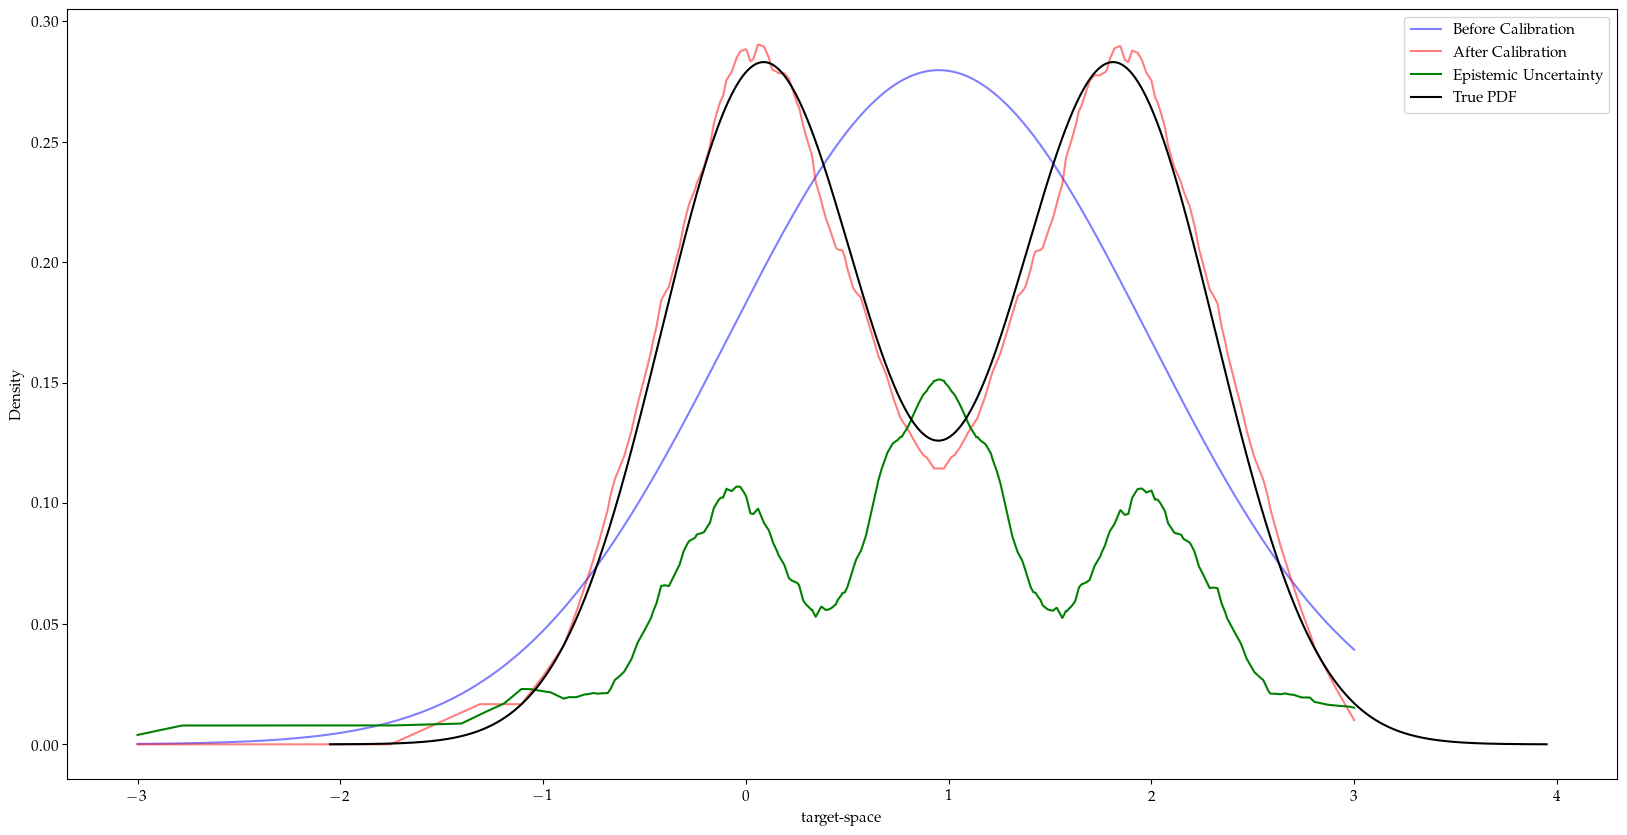
\includegraphics[width=0.8\textwidth]{resources/recalibration_bimodal_cde.png}
    \caption{Recalibration of a bimodal CDE model. The model is recalibrated by shifting the quantiles of the HDR.}
    \label{fig:recalibration}
\end{figure}

A Pseudo Code where we use HDR to recalibrate a CDE model is provided in \sref[Algorithm]{alg:calibrate_pdf}.

\section{Uncertainty and Calibration: The Connection}\label{sec:uncertainty_calibration}

The general area of uncertainty estimation has been growing drastically in recent years. This is because of the increasing complexity of models and the need to understand the models better as well as the requirement in risk-sensitive applications to understand when and how much the model can be trusted. Generally, as described by \cite{hullermeier_aleatoric_2021} there exist a lot of different types and perspectives on uncertainty. Most importantly there exists a distinction between so called aleatoric and epistemic uncertainty. Not all defintions of those two fully agree but generally aleatoric uncertainty is the inherent stochtasticity of the data while epistemic uncertainty is the unsureness of the model if only a limited amount of data is observed.

For example, if we try to model the coinflip of a biased coin with 75\% probability of landing on the head and 25\% on tails, then epistemic uncertainty would be if we did only observe 10 coinflips and we are unsure yet about the exact porbabilities within the coin. Aleatoric uncertainty would be the the inherent randomness of the coin that we might try to model. This means the 75\% and 25\% themselves are the aleatoric uncertainty.
Differences of interpretation of those two kinds of uncertainty are in practice often inherent in how we expect the true model of the data to be and how it really is. For example, if we were to expect for the coinflip experiment that the coin is always landing on the same side with the intention to learn this side,and differences in what we observe is simply noise, then we might not be able to model either uncertainty properly. In particular we might in this case predict that the coin always lands on head and there is simply 25\% noise which is of of course not true.
A slight variation in definitions between aleatoric and epistemic uncertainty within works \cite{hullermeier_aleatoric_2021} is often whether aleatoric uncertainty is only noise or if it also contains stochtasticity of the data that might be reducible with more features like hidden variables that are not really observable. In this work, we do not want to dive into the philosophical interpretation of this and define that aleatoric uncertainty is always the randomness of the targets, given a fixed set of features, without of considering that there might be hidden variables that actually could reduce this uncertainty.

CDE-methods' task is to model the aleatoric uncertainty when we try to predict targets given features. The CDE-method model $\mathcal{P}_\theta(x)$ that we estimate is supposed to come as closely as possible to the inherent randomness of the targets given the features. One particular aspect that rarely has been acknowledged is, that those models can, at least with the optimization objective alone, not learn epistemic uncertainty. This implies, that the model might actually give overestimations in the preciseness of outcomes. Moreover, since in this kind of setting model the aleatoric uncertainty itself and usually do not assume that there is such a thing as a second-order aleatoric uncertainty, we actually assume that the conditional distribution of a target given features is deterministic i.e. there is no (second-order) aleatoric uncertainty. This also directly implies that all error of a model which has certain asymptotic gurantees stems from epistemic uncertainty alone.

In this work we provide a novel perspective on how one can estimate full uncertainty which not only includes the directly modeled aleatoric uncertainty but also the epistemic uncertainty. In the context of CDE, aleatoric uncertainty asks the question how the targets are distributed, given the features, while epistemic uncertainty asks to which extent we can actually accurately predict that. Especially for CDE where we need to predict very specific details about the distribution of the data, this is a very important question, as we realistically in real world settings can never model the distribution with full accuracy.

The tool that we propose for this is a novel method that highlights calibration in a new way. In particular, we argue that recalibration of models can be used to accurately infuse the prediction with a lower bound on epistemic uncertainty. Thereby we can reestimate the whole distribution with both epistemic and aleatoric uncertainty which thus gives us a more accurate perspective on what we really know about the distribution of a target.

\subsection{All Model Error corresponds to Epistemic Uncertainty}\label{sec:uncertainty_calibration_connection}

Our proposed method relies on two key insights. First, all error in CDE-method models is exclusively due to epistemic uncertainty if the model is asymptotically correct and does not over-/underfit. Secondly, if we observe that a model is miscalibrated, it is a direct implication that the model is suboptimal and thus that there is error. In particular what that tells us is, if a model is misaclibrated there is epistemic uncertainty. Moreover, we claim that the amount of miscalibration is in a direct relationship with the amount of epistemic uncertainty and we also claim that if we can recalibrate the whole model, we can estimate a lower bound of the epistemic uncertainty as the difference between the distribution of the uncalibrated and the calibrated model.

In order to solidify those claims and insight we need to define a variant of epistemic uncertainty where we can show those relationships. In particular, in our case we aim to express the amount of epistemic uncertainty in the output space of the model, i.e. in the space of the conditional PDF that we estimate. Therefore we observe that it is a fair statement to say that if the likelihood of the data given the model increases, the model is closer to the true model. The reason why this insight is non-trivial in the context of CDE-methods is that we generally do not have information about the optimal likelihood that could be obtained which is due to the fact that we need to make smoothness assumptions as described in \pef{sec:smoothness} and have limited data.

\begin{lemma}\label{lem:likelihood_increase_calibration}
    If we have a model $\mathcal{P}_{\theta}$ that is miscalibrated w.r.t. HDR on $\mathbf{Z}_I$, then there must exist a model $\mathcal{P}_{\theta'}$ that is calibrated and where we have a higher likelihood if the true $p(\mathbf{Y}\mid\mathbf{X})$ fullfills \sref[Assumptions]{def:assumptions}.
\end{lemma}

\begin{proof}
    %TODO
\end{proof}
% \begin{proof} %its wrong because M might be dependent on each x/the model
%     Miscalibration of $\mathcal{P}_\theta$ means that there exists a region in this restricted set that has a different probability mass than $\mathcal{Z}$ on this region. Specifically, this means that there is a subset of the target space that might depend on $\mathbf{X}$ where all elements of $\mathcal{P}_\theta$ in this region have a different probability mass than the true mass in expectation over $\mathbf{X}$. Let $M(\mathbf{X})$ be this subset of the target space. We have:

%     \begin{equation}
%         \exists M \in \mathbb{R}^n \to \mathbb{B}(\mathbb{R}^m) \forall p \in \mathcal{P}_\theta: \mathbb{E}_\mathbf{X}\left[\right|\int_{M(\mathbf{X})} p(y) dy\right] \neq \mathbb{E}_\mathbf{X}\left[ \int_{M(\mathbf{X})} p_{\text{true}}(y) dy \right] =: p_M
%     \end{equation}

%     % That is like an even harder version of the thing I already did before... I need to think about this more. Maybe just use HDR and be done with it.

%     We can see that there must be a region around each interval in $M$ such that any additional but small region is still miscalibrated. Rigorously, if we have an $M$ where we are miscalibrated, then we can write $M = \Cup_{i=1}^\infty M_i$, i.e. we can write $M$ as a countable union of disjoint intervals (or connected regions with $m > 1$) which follows since we are working on a Borel $\sigma$-algebra. Here now continuity implies that for a small $\epsilon$ we can find an inner/outer region round each $M_i$ such that the mass on the true probability is changed by $\epsilon$. This is because of the assumptions on $p$.

% \end{proof}

\sref[Lemma]{lem:likelihood_increase_calibration} shows us that if we are not calibrated than we know that we still have an error in the model i.e. that we have epistemic uncertainty to some extent. Moreover, it shows that if we racalibrate the model, it will have less epistemic uncertainty and so the difference between the recalibrated and the uncalibrated model is a lower bound on the epistemic uncertainty that we have for the problem at hand. In particular, one way to quantify this epistemic uncertainty is to use distributional measures of difference like the average Hellinger Distance, KL-divergence or the Wasserstein distance.

This measuring of epistemic uncertainty works if we assume smoothness in the true model, in particular in way that if we have a wrong model and we shift its quantiles, which is what we are doing when recalibrating, that intermediate results of this transition of quantiles are smoothly related to the optimization alogorithm itself. In particular, this is true since we assume that the model does not overfit and thus the model must be to some extent smooth w.r.t. epsitemic uncertainty, i.e. it will not have sharp edges in the distribution of the targets and, in particular, it approaches the true distribution in a smooth way from a less sharp distribution. For a more detailed understanding on the relation between overfitting and smoothness we refer to the work of \cite{bishop2006pattern}.

\chapter{Empirical Study}\label{chap:empirical_study}

In order to practically verify the validity of the novel theoretical findings as described in \pef{sec:cp_sub_cde} and the approach to use the HDR as described in \pef{sec:optimal_cp} for finding the best conformal regions we did a series of experiments with two different stages and a multitude of benchmark datasets. In particular, the first stage was a extensive hyperparameter search with Bayesian optimization on eight datasets with over 1000 hyperparameter configurations on each. Thereby nested cross validation was utilized. The goal of this stage was to get a better understanding of the hyperparameters, including novel hyperparameters and to find a good starting point for the next stage. The second stage then was to do a more detailed hyperparameter search with a smaller grid but with multiple test set splits to get a better understanding of the generalization of the hyperparameters. In this chapter we will describe the results of the first stage and the setup of the second stage. In particular we will discuss mutliple novel hyperparameters that we experimented with and highlight the ones that significantly improved the performance of the models empirically.

\section{Core Model Classes}\label{sec:core_model_classes}

In the course of this work we experimented with a multitude of different CDE-method model classes. In particular, insights gained from \pef{sec:cp_sub_cde} establish that we can use any model class in the literature that has been used from CDE, QR or CP which opens up a wide range of options. Model classes experimented with in this work include Mixture Density Networks (MDNs) by \cite{bishop1994mixture}, Kernel Mixture Networks (KMNs) \cite{ambrogioni2017kernel}, Multiple Quantile Regression (MQR) \cite{gupta2022nested,moon2021learning}, Normalizing Flow Networks (NFNs) by \cite{trippe2018conditional} and conventional Regression as a baseline. However, in the latter experimental stages we restricted ourselves to MDNs, KMNs and MQRs as they showed the best performance in the first stage and also have significantly lower computational requirements than NFNs which is also why we restrict the reports to those three model classes in this work.

\section{Experimental Setup}\label{sec:experimental_setup}

For the experiments done in the course of this work a python setup with standard libraries like PyTorch \cite{paszke2019pytorch}, NumPy \cite{harris2020array}, Pandas \cite{reback2020pandas}, Scikit-Learn \cite{scikit-learn} and others was utilized. The hardware consisted of NVIDIA TITAN X (Pascal) GPUs, each with 12GB memory.

\section{Hyperparameters}\label{sec:hyperparameters}

Architectures in this regime of ML offer an extremely wide range of possible hyperparameter settings. In particular, this is due to the fact that in the output space there is a lot of freedom in how we can model the distribution. While not the main focus of this work, it is an interesting realization that CDE-methods have possibly the most degrees of freedom in their output compared to any other ML task. In particular, it is impossible to fully output in all those degrees of freedom but any output must necissarly be an abstraction of the true PDF. For example we just output model parameters of a mixture of Gaussians instead of the infinitely dense PDF which is very obviously not possible. The elegance now comes in how we decide to make this abstractions and many options with the help of CDE-methods exist.

In this section first we will discuss the known hyperparameters and how the performance seems to be affected by them with a rigorious empirical analysis of good settings for those in the regime of CDE-methods. Then we will discuss novel hyperparameters that we experimented with and how they affected the performance of the models. In particular we found that there is no existing literature that discusses in depth the possible hyperparamters for CDE-methods and their impact. This is a very important contribution of this work as it gives a good starting point for future research in this area as well as a good starting point for practical applications of CDE-methods in the industry.

\subsection{Known Hyperparameters - General}

\subsubsection{Learning Rate}

A learning rate of around \texttt{2e-4} gave us good performance accross all datasets. Moreover, for some of our experiments we utilized a learning rate scheduler \texttt{ReduceLROnPlateau} with a patience of $5$ epochs, cooldown of $3$ and a factor of $0.5$. This gave us a slight performance boost when using MDN and KMN models, but not with MQR models.

\subsubsection{Batch Size}

This hyperparameter varies a lot between datasets. Some datasets had a better performance with a size around $32$ and others performed best with as high as $512$ with a significant impact on performance. We suggest that this hyperparameter should be tuned for each dataset individually. We did not experiment with a batch size scheduler.

\subsubsection{Number of Epochs}

We found the models had a rather quick convergence with mostly lower than $50$ epochs and performance not improving with more epochs. Furthermore we used early stopping by monitoring the negative log likelihood loss for all models as this loss is the most important one for CDE-methods.

\subsubsection{Dropout}

We experimented with a wide range of dropout rates and found that the models are extremely sensitive to this hyperparameter. In particular a dropout rate of more than $0.05$ will lead to a significant performance decrease for most instances. However, there are some exceptions, in particular when using KMN. Moreover we observed a correlation between the Dropout rate, number of components in MDN, number of layers and number of units. A more expressive architecture allows for a slight increase in dropout which is to be expected. Moreover, we suspect that the higher dropout preference in KMN is due to the reduced degrees of freedom in the KMN model compared to MDN and MQR.

\subsubsection{Weight Decay}

We initially did experiment with this hyperparameter, tuning it in many ways. However, we found that setting it to $0$ consistently yields the best performance.

\subsubsection{Base Architecture}

The base architecture used was a multi layer perceptron (MLP). We experimented with a wide range of depths and widths and the most performant architecture was one with four hidden layers with sizes $[64, 128, 128, 64]$; however it is possible that with significantly more or complex data a deeper architecture might be beneficial.

\subsubsection{Activation Function}

The different activation functions we tried were ReLu, Leaky ReLu, TanH, Sigmoid, SELU and ELU. The three best performing ones were ReLu, Leaky ReLu and TanH, however, the differences were not very significant and there are some slight variations between datasets. We decided to use ReLu as it was the most stable one. It is noteworthy that when using ReLu we utilized a He initialization and when using TanH we utilized a Xavier initialization as best practice.

\subsubsection{Input-/Output Noise}

A hyperparamter that to the best of our knowledge is novel to the CP model literature and was first introduced to CDE methods by \cite{rothfuss2019noise} is the input/output noise to the models. This hyperparameter boosts the performance very significantly and it essential for performance in all CDE-methods. We found an input and output noise of around $0.03$ the most consistent, however, tuning this hyperparameter for each dataset can improve the performance even further by a significant margin. In particular when using KMN a higher noise level is sometimes beneficial with values up to $0.3$.

\subsubsection{Layer Norm}

Layer Norm was tried in the later course of the experiments and we found it does reduce the performance of all our models. We did not investigate this further.

\subsubsection{Component Entropy Loss}

This additional regularization loss which can be used in MDNs and KMNs essentially aims to decrease the entropy of the different mixture components. We found adding a small amount of around $0.125$ tends to slightly increase the performance of the models.

\subsubsection{Number of Components}

The number of components in both MDN and KMN make a significant difference. For MDN a number of components around $35$ was the most performant across all datasets. For KMN a higher number of $90$ was the best performing one. Moreover, we we had two kernels in the KMN model. This makes an effective number of components of $180$. For MQR generally a higher quantile number is better always since with a higher number basically we can model the conditional CDF better. However, we restricted ourselves to $256$.

\subsubsection{Component Distribution}
We experimented with Laplacian and Gaussian mixture components. Both have their advantages and disadvantages depending on the dataset. However, the differences were not very big and since Gaussian components were slightly more performant we decided to use those.

\subsubsection{Kernel Width}
We initialized the kernel width with $0.3$ and $0.7$ but decided to make them learnable hyperparameters, which means that we optimize them with the model parameters which slightly boosted the performance.

\subsection{Novel Hyperparameters}

\subsubsection{Additional Target Noise}

As explained in the theoretical part of this work, in order to be a reasonable prediction that can also be calibrated effectively, certain conditions need to be fullfilled on the distributions. In particular, it is required to have a certain amount of density everywhere. Moreover, we suspected that it might be helpful to enforce the marginal target distribution component on the CDE-models since then during calibration we can be sure that for each possible target there is at least a small amount of density in the model. In particular we decided to implement this by swapping certain targets which implicitly should enforce that the model has a certain amount of density everywhere on the marginal distribution. Furthermore, a theory was that if we have more samples then we have less empistemic uncertainty which implies that we would need to inforce less density on the marginal distribution and thus we made the number of swaps per epoch.

Another suspicion, especially for MDNs, was that some components can never "reach" the density where they want to go during training. In particular this came from the assumption, that if initially all mixture componens are somewhat in the center and we have a smaller density more on an outside location, that in order for a component to move to this location it would need to bridge the gap betweeen the high density in the center to the lower peak on the outside which might be very low density. We suspected that if a component needs to do that it might cause degenerative behaviour since if a component is at a location with low actual density the loss should enforce a lower weight on the component, which, in turn will decrease the general gradient imposed on this component. We suspected that it might happen that a component will then just stay in a gap with a negicible amount of weight so that it will never move again. In order to counteract this we decided to initialize the training with a large amount of uniform noise in the space of the targets and let it decay rather quickly over time. This procedure slightly improved the performance on all tasks but it is hard to say if there might be better ways to do it.

\subsubsection{Learn MQR Quantile Distribution Std}

MQR asymptotically with an increase in quantile components can as shown in \pef{sec:cp_sub_cde} model the true PDF fully. However, since we have a limited amount of training data and also a limited amount of compute we needed to resrict the number of components to $256$. In order to still be able to efficiently calculate the density at a point we decided to treat each quantile as a component with equal weight in a mixture of gaussians. Thereby we decided to learn the standard deviation. However, the standard deviation in this case can not be learned with the Pinball loss that is used for MQR. Thus we decided to use the NLL loss for the standard deviation only but without impacting the quantiles. We did this by detaching the means from the computational graph of the gradient in the loss function.

\section{Datasets}

In the course of this work we experimented with a multitude of different datasets. In particular, we tried to orient ourselves at the literature in CP and CDE \cite{rothfuss2019noise,sesia2021conformal} and used most of the datasets that were used there. Moreover we tried to have datasets with some different properties to gain more insight into strenghts and weaknesses of different models. Thereby we used \texttt{Boston Housing}, \texttt{Concrete}, \texttt{Energy Efficiency} as smaller datasets in order to elaborate performance with lower number of samples. Moreover, we used larger datasets \texttt{Meps19}, \texttt{Meps20}, \texttt{Meps21}, \texttt{CASP}, \texttt{Blog}, \texttt{Facebook1}, \texttt{Facebook2}. Finally, we used two versions of a time series dataset provided by VoestAlpine AG about energy price prediction. In particular \texttt{VoestRealistic} and \texttt{VoestIdeal} are two variations of the same data where we used realistic features and features as if we could look into the future respectively. This dataset was used to investigate the performance of CDE-methods on time series data.\footnote{The features used for the Voest datasets were all taken from \url{https://transparency.entsoe.eu/dashboard/show} in a time windows from November 2022 till November 2023 but will not be directly disclosed.} In \tef{tab:dataset_overview} we provide an overview of the characteristics of each dataset.

\begin{table}
    \caption{Comparison of Different Used Datasets}
    \label{tab:dataset_overview}
    \centering
    \begin{tabular}{lrrr}
        \toprule
        Dataset        & \# Samples & \# Features & Description                      \\
        \midrule
        Boston Housing & 506        & 13          & Housing prices in Boston         \\
        Concrete       & 1030       & 8           & Concrete compressive strength    \\
        Energy         & 768        & 8           & Energy efficiency of buildings   \\
        CASP           & 45730      & 9           & Protein structure prediction     \\
        Blog           & 52397      & 280         & Blog popularity prediction       \\
        Facebook1      & 40948      & 53          & Facebook user engagement         \\
        Facebook2      & 81311      & 53          & Facebook user engagement         \\
        Meps19         & 15785      & 139         & Medical Expenditure Panel Survey \\
        Meps20         & 17541      & 139         & Medical Expenditure Panel Survey \\
        Meps21         & 15656      & 139         & Medical Expenditure Panel Survey \\
        VoestRealistic & 35001      & 42          & Realistic Features Voest Dataset \\
        VoestIdeal     & 35001      & 42          & Ideal Features Voest Dataset     \\
        \bottomrule
    \end{tabular}
\end{table}

\section{Calculation of the HDR}

Calculating the HDR is a straightforward procedure which is described in the PseudoCode below in \sref[Algorithm]{alg:hdr} where we assume that the target grid is spaced equally but that is not required technically. The output are the elements of the target grid that are in the HDR. To obtain the actual intervals we just need to go half the step size to the left and right of each element in the HDR but it is left out the algorithm for inconvenience of writing that down. Moreover it is possible to add an improvement step into \sref[Algorithm]{alg:hdr} where we can smooth the HDR via linear interpolation between the consecutive densities. This is a very important step as it can significantly improve the performance of the models in particular if it is expensive to evaluate the density at each point by using the model itself. Moreover when we want a single interval as region than as argued in \pef{sec:density_focus} we just connect the largest and smallest border of the HDR which is guranteed to have more than $\alpha$ probability mass. Note that if we have after the $I_{HDR} + 1$ item other items that have the same density as the $I_{HDR} + 1$ item technically also should include those in the HDR but we decided to not do that for simplicity.

\begin{algorithm}
    \caption{HDR Calculation}
    \label{alg:hdr}
    \begin{algorithmic}
        \STATE \textbf{Input:} CDE-method model $f$, Features $x$, Significance Level $\alpha$, Target Grid $y$
        \STATE \textbf{Output:} HDR $H$

        \STATE $p \leftarrow f(x, y)$
        \STATE $p_{\text{normalized}} \leftarrow \frac{p}{\text{sum}(p)}$ We normalize the density
        \STATE $I_{\text{sorted}} \leftarrow \text{argsort}(p_{\text{normalized}})[::-1]$ We sort in descending order
        \STATE $p_{\text{sorted}} \leftarrow p_{\text{normalized}}[I_{\text{sorted}}]$
        \STATE $p_{\text{cumsum}} \leftarrow \text{cumsum}(p_{\text{sorted}})$
        \STATE $I_{\text{HDR}} \leftarrow \text{sum}(p_{\text{cumsum}} < 1 - \alpha)$ We look how many elements we need to take
        \STATE $H \leftarrow y[I_{\text{sorted}}[:I_{\text{HDR}} + 1]]$ We take the elements in the HDR on the overestimated side

        \RETURN $H$
    \end{algorithmic}
\end{algorithm}

\section{Calculating the Calibrated Conditional PDF}

For calibrating the whole PDFs of a dataset we need to find the adjustment for a grid of quantile levels similar to how we would do it for calibrating CP for a sigle level. Therefore we can use \sref[Algorithm]{alg:calibrate_pdf} below which expects calibration samples. In practice we observed that even when inputting the training samples for calibration it increases the general performance. Moreover, it is almost necessary to do smoothing because otherwise the result will be very noisy. In the second for loop we basically reconstruct the PDF from the calibrated HDR by assigning each HDR level the same density. Even tho this algorithm will marginally increase the performance it is possible that on single samples the performance is significantly worse. Moreover, we can obtain a quantification of the epistemic uncertainty by integrating the returned value.

\begin{algorithm}
    \caption{Calibrating a HDR at a specific level}
    \label{alg:calibrate_hdr}
    \begin{algorithmic}
        \STATE \textbf{Input:} Density Grids $p$, Calibration Targets $y$, Significance Level $\alpha$, Target Grid $\bar{y}$
        \STATE \textbf{Output:} Calibrated Significance Level $\alpha'$

        \STATE $p_{\text{normalized}} \leftarrow \frac{p}{\text{sum}(p)}$ We normalize the density
        \STATE $I_{\text{sorted}} \leftarrow \text{argsort}(p_{\text{normalized}})[::-1]$ We sort in descending order
        \STATE $p_{\text{sorted}} \leftarrow p_{\text{normalized}}[I_{\text{sorted}}]$
        \STATE $\text{cumsum} \leftarrow \text{cumsum}(p_{\text{sorted}})$
        \STATE $\hat{alpha} \leftarrow \text{cumsum}[\argmin(|p_{\text{cumsum}} - \alpha|)]$ We find the required quantile levels

        \STATE $\alpha' \leftarrow 1 - \text{quantile}(\hat{alpha}, 1 - \alpha)$ We find the quantile level of the closest level

        \RETURN $\alpha'$

    \end{algorithmic}
\end{algorithm}

\begin{algorithm}
    \caption{Calibrating the Conditional PDF}
    \label{alg:calibrate_pdf}
    \begin{algorithmic}
        \STATE \textbf{Input:} CDE-method model $f$, Calibration Features $x$, Calibration Targets $y$, Significance Level Grid $\alpha$, Target Grid $\bar{y}$
        \STATE \textbf{Output:} Calibrated Conditional PDF grid $p'$, Epistemic Uncertainty $p_e$

        \STATE $p \leftarrow f(x, \bar{y})$
        \STATE $\bar{y}_{\text{spacing}} \leftarrow \bar{y}[1] - \bar{y}[0]$

        \FOR{$\alpha_i$ in $\alpha$}
        \STATE $\alpha'_i \leftarrow \text{HDR-Calibrate}(p, y, \bar{y}, \alpha_i)$ Here we use \sref[Algorithm]{alg:calibrate_hdr} to calibrate the HDR
        \STATE $H_i \leftarrow \text{HDR}(p, \alpha'_i, \bar{y})$
        \ENDFOR

        \STATE $H_0 \leftarrow \emptyset$
        \STATE $H_{N+1} \leftarrow \text{ones}(\text{len}(\bar{y}))$
        \FOR{$i$ in $1, \dots, \text{len}(\alpha) + 1$}
        \STATE $H_i \leftarrow H_{i - 1} \cap H_i$ We take the intersection of the HDRs to get the elements for this level
        \STATE $p'[H_i] \leftarrow \frac{1}{\text{len}(\alpha) \cdot \text{sum}(H_i) \cdot \bar{y}_{\text{spacing}}}$ We adjust the density for the elements in the HDR
        \ENDFOR

        \STATE $p_e \leftarrow \text{p - p'}$ We calculate the epistemic uncertainty grid

        \STATE $p' \leftarrow \text{smooth}(p')$ Optional smoothing because of finite samples and finitely fine grids
        \STATE $p_e \leftarrow \text{smooth}(p_e)$ Optional smoothing because of finite samples and finitely fine grids

        \RETURN $p', p_e$
    \end{algorithmic}
\end{algorithm}

\section{Experiment Results} \label{sec:results}

\subsection{Recalibration of the Whole CDE}

We incoperate recalibration of the whole CDE in some of our experiments (not all due to time-constraints) where we can observe also an increase in performance on real world datasets. In particular by choosing the smoothing window appropriately we can consistently increase the performance on validation sets even when calibrating on the train set itself which shows the utility of this method. \fef{fig:recalibration_concrete} shows examples of recalibration on the concrete dataset where we smooth with $\frac{1}{16}$ of the grid size. In terms of likelihood, the recalibrated method shows a slight but significant increase in likelihood on the test set, in particular $-3.202$ instead of $-3.224$ in average log likelihood. %TODO add more rigorous results (multi-seed etc)

\begin{figure}
    \centering
    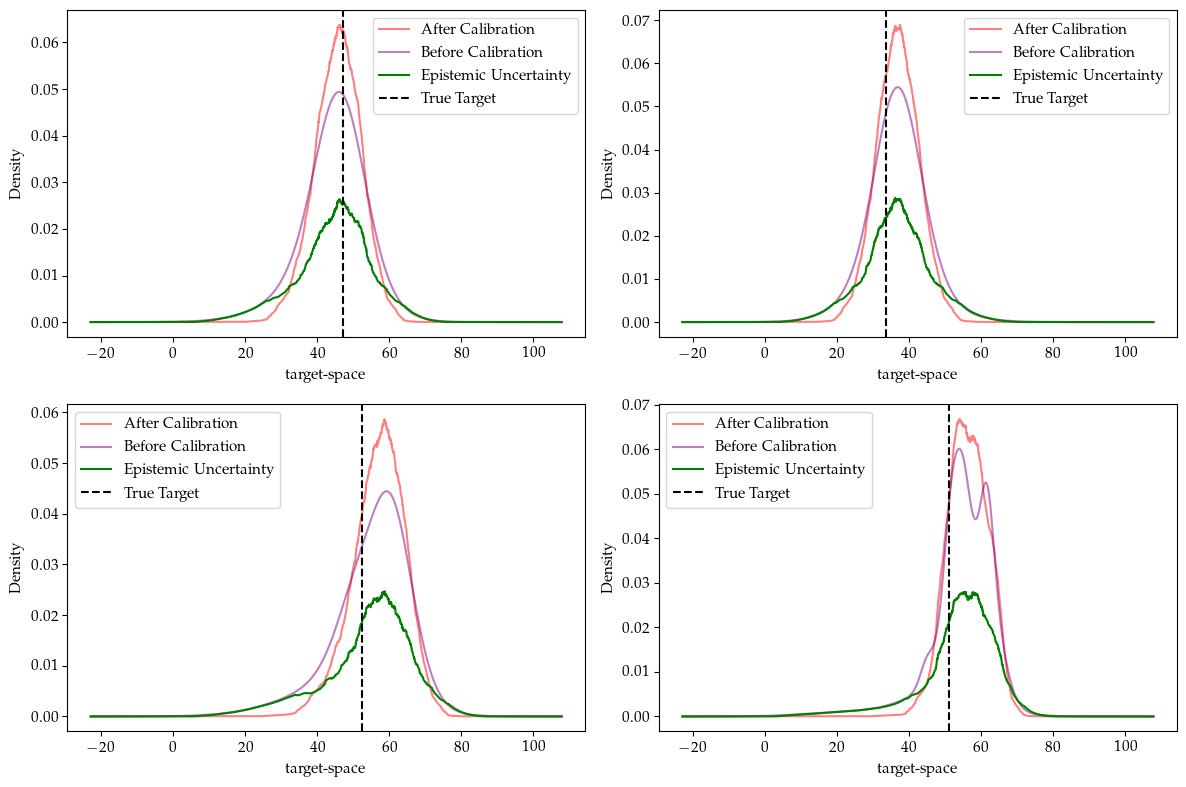
\includegraphics[width=0.8\textwidth]{resources/recalibration_concrete_dataset.png}
    \caption{Recalibration of the whole estimated conditional PDF on the Concrete dataset. Calibrated on the train dataset and evaluated on the test dataset.}
    \label{fig:recalibration_concrete}
\end{figure}

Moreover, we can observe that recalibration of the full CDE can empirically compensate for a significant amount of model misspecification. In particular, as we can also see in \fef{fig:recalibration} where the model was specified as an unimodal gaussian distribution but the true distribution is multimodal. In this case the recalibration can compensate for the misspecification as can even recover the bimodal distribution which makes it more than just a nice utility but a powerful tool that can be used to compensate and potentially identify model misspecification.

\subsection{Main Benchmark Results}
Here we show the results of the final experiments on the 12 datasets. The main experimental procedure consisted for each dataset except for the two Voest ones of five-fold nested cross validation to obtain a robust estimate of the actual performance. On the two Voest Datasets instead we decided to always use the same train-test split where we consider the time dependence in the data by using the chronologically first 80\% of the data as training data and the last 20\% as test data. For the other datasets we used 80\%-20\% train-test spilts which is notably different from \cite{sesia2021conformal} who used a fixed test set of 2000 samples, 2000 for calibration and the other part for training. In particular, on all datasets that we have the same, we have signlificantly less train dat but still competitive results.  Moreover, we do cross-validation on a time series split where we expand the training data and use the chronolocially last part for validation. For the exact implementation we refer to our code. The Algorithm used for the evaluation can be seen in \sref[Algorithm]{alg:evaluation}. This algorithm inspired by \cite{rothfuss2019noise} is a nested cross validation algorithm over multiple seeds and hyperparameters that gurantees a robust estimate of the performance of the models on the test set. In particular, the test set is only used for the final evaluation and the hyperparameters are tuned on the training set which we do CV on.

The results final benchmark results are shown in \tef{tab:results_interval_size_hdr} and \tef{tab:results_interval_size_hdr_connected}. As expected, resuls in the table with connected intervals are only slightly larger than the true HDR. Comparing our results to the current state of the art which is \cite{sesia2021conformal} to our best knowledge, we can see that mostly we beat the results with pure HDR and even in some instances like the CASP dataset when using connected intervals which proofs that our methods and hyperparameters are very competitive. 

\begin{algorithm}
    \caption{Evaluation of the Models}
    \label{alg:evaluation}
    \begin{algorithmic}
        \STATE \textbf{Input:} Hyperparameter Grid $H$, Model Class $M$, Dataset $D$, Number of Folds $K$, Number of Nested Folds $L$
        \STATE \textbf{Output:} Performance Metrics $P$

        \FOR{$k$ in $1, \dots, K$}
        \STATE $D_{\text{train}, k}, D_{\text{test}, k} \leftarrow \text{split}(D, k)$

        \STATE $CVSplits \leftarrow \text{split}(D_{\text{train}, k}, L)$

        \FOR{$h$ in $H$}
        \FOR{$D'_{\text{train}} D'_{\text{val}}$ in $CVSplits$}
        \STATE $M_h \leftarrow \text{fit}(M, D'_{\text{train}}, h)$
        \STATE $P_h \leftarrow \text{score}(M_h, D'_{\text{val}})$
        \ENDFOR
        \ENDFOR

        \STATE $h_{\text{best}} \leftarrow H[\text{argmax}(P)]$ Also set calibrated hyperparameters like epoch and $\alpha$ for CP

        \STATE $P_k \leftarrow \text{fit}(M, D_{\text{train}}, h_{\text{best}})$
        \STATE $P_k \leftarrow \text{score}(M_k, D_{\text{test}})$
        \ENDFOR

        \STATE $P \leftarrow \text{mean}(P)$

        \RETURN $P$
    \end{algorithmic}
\end{algorithm}

\begin{table}[h!]
    \centering
    \caption{CDE Experiment Result CP with HDR Interval Size (lower is better)}
    \label{tab:results_interval_size_hdr}
    \begin{tabular}{l*{3}{d{3.8}}}
        \toprule
        \multicolumn{1}{c}{Dataset} & \multicolumn{1}{c}{MDN} & \multicolumn{1}{c}{KMN} & \multicolumn{1}{c}{MQR} \\
        \midrule
        Boston Housing              & 9.45 \pm 0.70           & 9.79 \pm 0.35           & 9.32 \pm 0.37           \\
        Concrete                    & 19.72 \pm 0.71          & 19.37 \pm 0.97          & 17.56 \pm 0.55          \\
        Energy                      & 6.26 \pm 0.18           & 3.99 \pm 0.28           & 3.89 \pm 0.27           \\
        CASP                        & 8.41 \pm 0.17           & 7.81 \pm 0.15           & 9.47 \pm 0.18           \\
        Blog                        & 11.96 \pm 0.76          & 11.83 \pm 0.72          & 12.46 \pm 0.77          \\
        Facebook 1                  & 12.19 \pm 0.64          & 11.33 \pm 0.64          & 11.34 \pm 0.53          \\
        Facebook 2                  & 12.81 \pm 1.72          & 12.02 \pm 1.69          & 12.18 \pm 1.55          \\
        Meps 19                     & 19.41 \pm 1.59          & 19.49 \pm 1.22          & 21.13 \pm 1.22          \\
        Meps 20                     & 19.26 \pm 1.00          & 18.53 \pm 0.96          & 19.98 \pm 0.89          \\
        Meps 21                     & 19.02 \pm 1.17          & 18.85 \pm 0.87          & 20.65 \pm 0.78          \\
        \bottomrule
    \end{tabular}
\end{table}

\begin{table}[h!]
    \centering
    \caption{CDE Experiment Result CP with HDR Connected Interval Size (lower is better)}
    \label{tab:results_interval_size_hdr_connected}
    \begin{tabular}{l*{3}{d{3.8}}}
        \toprule
        \multicolumn{1}{c}{Dataset} & \multicolumn{1}{c}{MDN} & \multicolumn{1}{c}{KMN} & \multicolumn{1}{c}{MQR} \\
        \midrule
        Boston Housing              & 9.60 \pm 0.77           & 10.23 \pm 0.55          & 9.32 \pm 0.37           \\
        Concrete                    & 19.88 \pm 0.72          & 19.39 \pm 0.96          & 17.56 \pm 0.55          \\
        Energy                      & 6.53 \pm 0.23           & 4.22 \pm 0.29           & 3.89 \pm 0.27           \\
        CASP                        & 11.29 \pm 0.26          & 11.05 \pm 0.20          & 10.27 \pm 0.26          \\
        Blog                        & 12.12 \pm 0.77          & 17.89 \pm 1.33          & 15.57 \pm 1.43          \\
        Facebook 1                  & 12.27 \pm 0.64          & 15.81 \pm 1.31          & 13.21 \pm 0.93          \\
        Facebook 2                  & 12.84 \pm 1.71          & 15.22 \pm 1.62          & 13.78 \pm 1.85          \\
        Meps 19                     & 19.86 \pm 1.66          & 29.67 \pm 2.40          & 22.90 \pm 1.59          \\
        Meps 20                     & 19.59 \pm 1.15          & 27.32 \pm 2.28          & 21.34 \pm 1.14          \\
        Meps 21                     & 19.75 \pm 1.46          & 28.31 \pm 1.72          & 22.37 \pm 1.14          \\
        \bottomrule
    \end{tabular}
\end{table}

\chapter{Conclusion}\label{chap:conclusion}



\chapter{ToDos}
1. Show that calibration is the same as in Gneiting et a. (probabilistic
calibration).
1a. Show that there are 2 sub-parts then for CP: fitting-calibration and
overfitting-calibration
Fitting Calibration: the model is probabilistically calibrated to the training
data (is fit well)
Overfitting Calibration: The model is basically the same way calibrated to the
training data as to the test data
-> time series and distributional differences come in here too but is a
further subchapter then

2. Then show what my recalibration method does mathematically and how it is
different from the other recalibration methods

This all contains that CP is a special case of CDE!

3. I should mention in the thesis the stages of my experiemnts. I first did
basically only the stuff I did in my practical work (but not sure if that
should even be mentioned). Then I should also mention that I did 1000 runs with
bayesian optimization on all datasets with a very high variable range of
possible hyperparameters with the goal to get a good understanding of the
hyperparameters (as there are some novel ones and complex ones). The next stage
that I will now start is the stage where I basically start with reasonably good
parameters infered by the previous runs and from there basically a. do very
specific experiments for the novel hyperparameters to find out there
effectiveness (small grid) b. do hyperparameter runs with a smaller grid but
multiple test set spilts (with nested cv).

4. As CP is a special case of CDE, also the synthetic reasoning that we
basically need them to make real statements about the performance of methods is
also valid for CP. So I should also mention that in the thesis. And from there
I can basically start finding out the best hyperparameters for CP methods and
then also do the same for CDE methods and also possibly new methods that defeat
ceavats on the synthetic sets that I only now can find out.

5. It might be interesting to look into the question if when there is some kind
of monotonicity between the hyperparameters and the performance of the model,
if that is a good synthetic dataset to infer strategies from. I think that is a
very interesting question and I should look into that. => "using hyperparameter
performances as a measure of the quality of a synthetic dataset."

6. Can I do more advanced recalibration strategies if the data is not IID?
(e.g. time series data)

->->-> After those are done its time to look into the strategy part where I
look how those CDE/CP can be practically used.